\documentclass[papersize,a4paper,12pt,uplatex]{jsarticle}
\usepackage{ketpic,ketlayer}
\usepackage{amsmath}
% \usepackage{amsmath,newtxmath}
\usepackage[dvipdfmx]{graphicx,color}
\usepackage{wrapfig}
\usepackage[dvipdfmx,bookmarks=false,colorlinks=true,linkcolor=blue]{hyperref}
\setmargin{20}{20}{15}{25}
\usepackage{setspace}
\usepackage{comment}
\setcounter{tocdepth}{3}

\begin{document}
\title{\ketcindy の概要}
\author{\ketcindy\ Project Team}
\maketitle

\begin{center}  - 第3.2版 -\end{center}
\hypertarget{index}{}
\tableofcontents

\newpage

\section{\ketcindy について}
\subsection{システムの構成}
\ketcindy は,Cinderella の作図機能を利用して,作図データの\LaTeX ファイルを作成するためのスクリプトライブラリである。\ketcindy はCinderellaのプログラミング言語Cindyscriptで記述されており,ユーザーはCinderella によるインタラクティブな作図機能と,CindyScript によるプログラミングを用いて,\LaTeX 文書の挿入図を効率よく作成することができる。また,各種数式処理ソフトと連携して計算を行うことができる。

\begin{center}
\scalebox{0.9}{ %%% /Users/Hannya/Desktop/KeTCindy/KeTCindyTools/fig/concept.tex 
%%% Generator=KeTCindy概念図.cdy 
{\unitlength=3.5mm%
\begin{picture}%
(39.08,22.04)(-24.72,-12.36)%
\special{pn 8}%
%
{%
\color[rgb]{0,1,0}%
\special{pa 1058 -568}\special{pa 1054 -627}\special{pa 1043 -686}\special{pa 1025 -742}%
\special{pa 999 -796}\special{pa 968 -846}\special{pa 930 -892}\special{pa 886 -933}%
\special{pa 838 -968}\special{pa 786 -996}\special{pa 731 -1018}\special{pa 673 -1033}%
\special{pa 614 -1041}\special{pa 555 -1041}\special{pa 495 -1033}\special{pa 438 -1018}%
\special{pa 383 -996}\special{pa 330 -968}\special{pa 282 -933}\special{pa 239 -892}%
\special{pa 201 -846}\special{pa 169 -796}\special{pa 144 -742}\special{pa 125 -686}%
\special{pa 114 -627}\special{pa 110 -568}\special{pa 114 -508}\special{pa 125 -450}%
\special{pa 144 -393}\special{pa 169 -339}\special{pa 201 -289}\special{pa 239 -243}%
\special{pa 282 -203}\special{pa 330 -168}\special{pa 383 -139}\special{pa 438 -117}%
\special{pa 495 -102}\special{pa 555 -95}\special{pa 614 -95}\special{pa 673 -102}%
\special{pa 731 -117}\special{pa 786 -139}\special{pa 838 -168}\special{pa 886 -203}%
\special{pa 930 -243}\special{pa 968 -289}\special{pa 999 -339}\special{pa 1025 -393}%
\special{pa 1043 -450}\special{pa 1054 -508}\special{pa 1058 -568}\special{sh 1}\special{ip}%
}%
{%
\color[rgb]{1,0,0}%
\special{pa 1940 -579}\special{pa 1937 -631}\special{pa 1927 -681}\special{pa 1911 -731}%
\special{pa 1889 -778}\special{pa 1861 -822}\special{pa 1828 -862}\special{pa 1790 -897}%
\special{pa 1748 -928}\special{pa 1703 -953}\special{pa 1654 -972}\special{pa 1604 -985}%
\special{pa 1553 -991}\special{pa 1501 -991}\special{pa 1449 -985}\special{pa 1399 -972}%
\special{pa 1351 -953}\special{pa 1305 -928}\special{pa 1263 -897}\special{pa 1226 -862}%
\special{pa 1193 -822}\special{pa 1165 -778}\special{pa 1143 -731}\special{pa 1127 -681}%
\special{pa 1117 -631}\special{pa 1114 -579}\special{pa 1117 -527}\special{pa 1127 -476}%
\special{pa 1143 -427}\special{pa 1165 -380}\special{pa 1193 -336}\special{pa 1226 -296}%
\special{pa 1263 -260}\special{pa 1305 -230}\special{pa 1351 -205}\special{pa 1399 -186}%
\special{pa 1449 -173}\special{pa 1501 -166}\special{pa 1553 -166}\special{pa 1604 -173}%
\special{pa 1654 -186}\special{pa 1703 -205}\special{pa 1748 -230}\special{pa 1790 -260}%
\special{pa 1828 -296}\special{pa 1861 -336}\special{pa 1889 -380}\special{pa 1911 -427}%
\special{pa 1927 -476}\special{pa 1937 -527}\special{pa 1940 -579}\special{sh 1}\special{ip}%
}%
{%
\color[cmyk]{0,0,0.5,0}%
\special{pa 1538 292}\special{pa 1535 243}\special{pa 1526 195}\special{pa 1510 148}%
\special{pa 1490 104}\special{pa 1463 62}\special{pa 1432 24}\special{pa 1396 -10}%
\special{pa 1356 -38}\special{pa 1313 -62}\special{pa 1267 -80}\special{pa 1220 -92}%
\special{pa 1171 -99}\special{pa 1122 -99}\special{pa 1073 -92}\special{pa 1025 -80}%
\special{pa 980 -62}\special{pa 937 -38}\special{pa 897 -10}\special{pa 861 24}\special{pa 830 62}%
\special{pa 803 104}\special{pa 782 148}\special{pa 767 195}\special{pa 758 243}\special{pa 755 292}%
\special{pa 758 341}\special{pa 767 389}\special{pa 782 436}\special{pa 803 481}\special{pa 830 522}%
\special{pa 861 560}\special{pa 897 594}\special{pa 937 623}\special{pa 980 646}\special{pa 1025 664}%
\special{pa 1073 677}\special{pa 1122 683}\special{pa 1171 683}\special{pa 1220 677}%
\special{pa 1267 664}\special{pa 1313 646}\special{pa 1356 623}\special{pa 1396 594}%
\special{pa 1432 560}\special{pa 1463 522}\special{pa 1490 481}\special{pa 1510 436}%
\special{pa 1526 389}\special{pa 1535 341}\special{pa 1538 292}\special{sh 1}\special{ip}%
}%
{%
\color[cmyk]{0,0,1,0}%
\special{pa 28 39}\special{pa 24 -9}\special{pa 11 -57}\special{pa -9 -103}\special{pa -36 -146}%
\special{pa -71 -187}\special{pa -112 -224}\special{pa -159 -257}\special{pa -212 -285}%
\special{pa -268 -308}\special{pa -329 -326}\special{pa -391 -338}\special{pa -455 -344}%
\special{pa -520 -344}\special{pa -584 -338}\special{pa -647 -326}\special{pa -707 -308}%
\special{pa -764 -285}\special{pa -816 -257}\special{pa -863 -224}\special{pa -905 -187}%
\special{pa -939 -146}\special{pa -967 -103}\special{pa -987 -57}\special{pa -999 -9}%
\special{pa -1003 39}\special{pa -999 87}\special{pa -987 134}\special{pa -967 180}%
\special{pa -939 223}\special{pa -905 264}\special{pa -863 301}\special{pa -816 334}%
\special{pa -764 362}\special{pa -707 385}\special{pa -647 403}\special{pa -584 415}%
\special{pa -520 421}\special{pa -455 421}\special{pa -391 415}\special{pa -329 403}%
\special{pa -268 385}\special{pa -212 362}\special{pa -159 334}\special{pa -112 301}%
\special{pa -71 264}\special{pa -36 223}\special{pa -9 180}\special{pa 11 134}\special{pa 24 87}%
\special{pa 28 39}\special{sh 1}\special{ip}%
}%
{%
\color[cmyk]{0,0.2,0,0}%
\special{pa -2458 39}\special{pa -2462 -5}\special{pa -2472 -47}\special{pa -2489 -88}%
\special{pa -2513 -127}\special{pa -2542 -164}\special{pa -2578 -197}\special{pa -2618 -227}%
\special{pa -2663 -252}\special{pa -2711 -273}\special{pa -2763 -289}\special{pa -2817 -300}%
\special{pa -2872 -305}\special{pa -2927 -305}\special{pa -2982 -300}\special{pa -3036 -289}%
\special{pa -3087 -273}\special{pa -3136 -252}\special{pa -3180 -227}\special{pa -3221 -197}%
\special{pa -3256 -164}\special{pa -3286 -127}\special{pa -3309 -88}\special{pa -3327 -47}%
\special{pa -3337 -5}\special{pa -3340 39}\special{pa -3337 82}\special{pa -3327 124}%
\special{pa -3309 165}\special{pa -3286 205}\special{pa -3256 241}\special{pa -3221 274}%
\special{pa -3180 304}\special{pa -3136 329}\special{pa -3087 350}\special{pa -3036 366}%
\special{pa -2982 377}\special{pa -2927 382}\special{pa -2872 382}\special{pa -2817 377}%
\special{pa -2763 366}\special{pa -2711 350}\special{pa -2663 329}\special{pa -2618 304}%
\special{pa -2578 274}\special{pa -2542 241}\special{pa -2513 205}\special{pa -2489 165}%
\special{pa -2472 124}\special{pa -2462 82}\special{pa -2458 39}\special{sh 1}\special{ip}%
}%
{%
\color[cmyk]{0.2,0.2,0,0}%
\special{pa -1298 39}\special{pa -1302 -5}\special{pa -1313 -47}\special{pa -1331 -89}%
\special{pa -1356 -128}\special{pa -1387 -164}\special{pa -1424 -198}\special{pa -1467 -228}%
\special{pa -1514 -253}\special{pa -1565 -274}\special{pa -1619 -290}\special{pa -1675 -301}%
\special{pa -1733 -306}\special{pa -1792 -306}\special{pa -1849 -301}\special{pa -1906 -290}%
\special{pa -1960 -274}\special{pa -2011 -253}\special{pa -2058 -228}\special{pa -2101 -198}%
\special{pa -2138 -164}\special{pa -2169 -128}\special{pa -2194 -89}\special{pa -2212 -47}%
\special{pa -2223 -5}\special{pa -2227 39}\special{pa -2223 82}\special{pa -2212 124}%
\special{pa -2194 166}\special{pa -2169 205}\special{pa -2138 242}\special{pa -2101 275}%
\special{pa -2058 305}\special{pa -2011 330}\special{pa -1960 351}\special{pa -1906 367}%
\special{pa -1849 378}\special{pa -1792 383}\special{pa -1733 383}\special{pa -1675 378}%
\special{pa -1619 367}\special{pa -1565 351}\special{pa -1514 330}\special{pa -1467 305}%
\special{pa -1424 275}\special{pa -1387 242}\special{pa -1356 205}\special{pa -1331 166}%
\special{pa -1313 124}\special{pa -1302 82}\special{pa -1298 39}\special{sh 1}\special{ip}%
}%
{%
\color[cmyk]{0.2,0,0.2,0}%
\special{pa -2458 1003}\special{pa -2462 960}\special{pa -2472 917}\special{pa -2489 876}%
\special{pa -2513 837}\special{pa -2542 801}\special{pa -2578 767}\special{pa -2618 738}%
\special{pa -2663 712}\special{pa -2711 691}\special{pa -2763 676}\special{pa -2817 665}%
\special{pa -2872 659}\special{pa -2927 659}\special{pa -2982 665}\special{pa -3036 676}%
\special{pa -3087 691}\special{pa -3136 712}\special{pa -3180 738}\special{pa -3221 767}%
\special{pa -3256 801}\special{pa -3286 837}\special{pa -3309 876}\special{pa -3327 917}%
\special{pa -3337 960}\special{pa -3340 1003}\special{pa -3337 1046}\special{pa -3327 1089}%
\special{pa -3309 1130}\special{pa -3286 1169}\special{pa -3256 1206}\special{pa -3221 1239}%
\special{pa -3180 1269}\special{pa -3136 1294}\special{pa -3087 1315}\special{pa -3036 1331}%
\special{pa -2982 1342}\special{pa -2927 1347}\special{pa -2872 1347}\special{pa -2817 1342}%
\special{pa -2763 1331}\special{pa -2711 1315}\special{pa -2663 1294}\special{pa -2618 1269}%
\special{pa -2578 1239}\special{pa -2542 1206}\special{pa -2513 1169}\special{pa -2489 1130}%
\special{pa -2472 1089}\special{pa -2462 1046}\special{pa -2458 1003}\special{sh 1}\special{ip}%
}%
{%
\color[cmyk]{0,0.1,0.3,0}%
\special{pa -1462 1003}\special{pa -1465 966}\special{pa -1475 930}\special{pa -1490 895}%
\special{pa -1512 861}\special{pa -1539 830}\special{pa -1571 801}\special{pa -1608 776}%
\special{pa -1649 754}\special{pa -1694 736}\special{pa -1741 722}\special{pa -1790 713}%
\special{pa -1840 709}\special{pa -1891 709}\special{pa -1941 713}\special{pa -1991 722}%
\special{pa -2038 736}\special{pa -2082 754}\special{pa -2123 776}\special{pa -2160 801}%
\special{pa -2192 830}\special{pa -2220 861}\special{pa -2241 895}\special{pa -2257 930}%
\special{pa -2266 966}\special{pa -2270 1003}\special{pa -2266 1040}\special{pa -2257 1077}%
\special{pa -2241 1112}\special{pa -2220 1145}\special{pa -2192 1177}\special{pa -2160 1205}%
\special{pa -2123 1231}\special{pa -2082 1252}\special{pa -2038 1270}\special{pa -1991 1284}%
\special{pa -1941 1293}\special{pa -1891 1298}\special{pa -1840 1298}\special{pa -1790 1293}%
\special{pa -1741 1284}\special{pa -1694 1270}\special{pa -1649 1252}\special{pa -1608 1231}%
\special{pa -1571 1205}\special{pa -1539 1177}\special{pa -1512 1145}\special{pa -1490 1112}%
\special{pa -1475 1077}\special{pa -1465 1040}\special{pa -1462 1003}\special{sh 1}\special{ip}%
}%
{%
\color[cmyk]{0,0.1,0.3,0}%
\special{pa 105 1240}\special{pa 102 1205}\special{pa 92 1171}\special{pa 76 1138}%
\special{pa 54 1107}\special{pa 26 1078}\special{pa -7 1051}\special{pa -45 1027}%
\special{pa -87 1007}\special{pa -133 990}\special{pa -182 977}\special{pa -232 969}%
\special{pa -284 964}\special{pa -336 964}\special{pa -388 969}\special{pa -438 977}%
\special{pa -487 990}\special{pa -533 1007}\special{pa -575 1027}\special{pa -613 1051}%
\special{pa -646 1078}\special{pa -674 1107}\special{pa -696 1138}\special{pa -712 1171}%
\special{pa -722 1205}\special{pa -725 1240}\special{pa -722 1275}\special{pa -712 1309}%
\special{pa -696 1342}\special{pa -674 1373}\special{pa -646 1403}\special{pa -613 1429}%
\special{pa -575 1453}\special{pa -533 1474}\special{pa -487 1490}\special{pa -438 1503}%
\special{pa -388 1512}\special{pa -336 1516}\special{pa -284 1516}\special{pa -232 1512}%
\special{pa -182 1503}\special{pa -133 1490}\special{pa -87 1474}\special{pa -45 1453}%
\special{pa -7 1429}\special{pa 26 1403}\special{pa 54 1373}\special{pa 76 1342}\special{pa 92 1309}%
\special{pa 102 1275}\special{pa 105 1240}\special{sh 1}\special{ip}%
}%
{%
\color[cmyk]{0,0.1,0.3,0}%
\special{pa 949 1033}\special{pa 945 996}\special{pa 935 959}\special{pa 918 923}%
\special{pa 895 889}\special{pa 866 857}\special{pa 831 828}\special{pa 792 802}\special{pa 748 780}%
\special{pa 701 762}\special{pa 650 748}\special{pa 598 738}\special{pa 544 734}\special{pa 490 734}%
\special{pa 436 738}\special{pa 383 748}\special{pa 333 762}\special{pa 285 780}\special{pa 241 802}%
\special{pa 202 828}\special{pa 167 857}\special{pa 138 889}\special{pa 115 923}\special{pa 99 959}%
\special{pa 88 996}\special{pa 85 1033}\special{pa 88 1071}\special{pa 99 1108}\special{pa 115 1144}%
\special{pa 138 1178}\special{pa 167 1210}\special{pa 202 1239}\special{pa 241 1265}%
\special{pa 285 1287}\special{pa 333 1305}\special{pa 383 1319}\special{pa 436 1329}%
\special{pa 490 1333}\special{pa 544 1333}\special{pa 598 1329}\special{pa 650 1319}%
\special{pa 701 1305}\special{pa 748 1287}\special{pa 792 1265}\special{pa 831 1239}%
\special{pa 866 1210}\special{pa 895 1178}\special{pa 918 1144}\special{pa 935 1108}%
\special{pa 945 1071}\special{pa 949 1033}\special{sh 1}\special{ip}%
}%
{%
\color[cmyk]{0,0.1,0.3,0}%
\special{pa -801 1348}\special{pa -804 1315}\special{pa -812 1283}\special{pa -827 1252}%
\special{pa -847 1223}\special{pa -873 1195}\special{pa -903 1170}\special{pa -937 1148}%
\special{pa -976 1129}\special{pa -1017 1113}\special{pa -1061 1101}\special{pa -1107 1093}%
\special{pa -1154 1089}\special{pa -1202 1089}\special{pa -1249 1093}\special{pa -1295 1101}%
\special{pa -1339 1113}\special{pa -1380 1129}\special{pa -1419 1148}\special{pa -1453 1170}%
\special{pa -1483 1195}\special{pa -1509 1223}\special{pa -1529 1252}\special{pa -1544 1283}%
\special{pa -1552 1315}\special{pa -1555 1348}\special{pa -1552 1380}\special{pa -1544 1412}%
\special{pa -1529 1443}\special{pa -1509 1472}\special{pa -1483 1500}\special{pa -1453 1525}%
\special{pa -1419 1547}\special{pa -1380 1566}\special{pa -1339 1582}\special{pa -1295 1594}%
\special{pa -1249 1602}\special{pa -1202 1606}\special{pa -1154 1606}\special{pa -1107 1602}%
\special{pa -1061 1594}\special{pa -1017 1582}\special{pa -976 1566}\special{pa -937 1547}%
\special{pa -903 1525}\special{pa -873 1500}\special{pa -847 1472}\special{pa -827 1443}%
\special{pa -812 1412}\special{pa -804 1380}\special{pa -801 1348}\special{sh 1}\special{ip}%
}%
{%
\color[cmyk]{0,0.4,0.3,0}%
\special{pa -606 -650}\special{pa -610 -684}\special{pa -619 -718}\special{pa -635 -751}%
\special{pa -657 -781}\special{pa -684 -810}\special{pa -717 -837}\special{pa -754 -860}%
\special{pa -795 -880}\special{pa -840 -896}\special{pa -887 -909}\special{pa -937 -918}%
\special{pa -987 -922}\special{pa -1038 -922}\special{pa -1089 -918}\special{pa -1138 -909}%
\special{pa -1186 -896}\special{pa -1230 -880}\special{pa -1272 -860}\special{pa -1309 -837}%
\special{pa -1341 -810}\special{pa -1369 -781}\special{pa -1390 -751}\special{pa -1406 -718}%
\special{pa -1416 -684}\special{pa -1419 -650}\special{pa -1416 -616}\special{pa -1406 -583}%
\special{pa -1390 -550}\special{pa -1369 -519}\special{pa -1341 -491}\special{pa -1309 -464}%
\special{pa -1272 -441}\special{pa -1230 -421}\special{pa -1186 -404}\special{pa -1138 -392}%
\special{pa -1089 -383}\special{pa -1038 -379}\special{pa -987 -379}\special{pa -937 -383}%
\special{pa -887 -392}\special{pa -840 -404}\special{pa -795 -421}\special{pa -754 -441}%
\special{pa -717 -464}\special{pa -684 -491}\special{pa -657 -519}\special{pa -635 -550}%
\special{pa -619 -583}\special{pa -610 -616}\special{pa -606 -650}\special{sh 1}\special{ip}%
}%
{%
\color[rgb]{0,0,0}%
\special{pa 1973 -193}\special{pa 1973 -232}\special{fp}\special{pa 1973 -271}\special{pa 1973 -310}\special{fp}%
\special{pa 1973 -350}\special{pa 1973 -389}\special{fp}\special{pa 1973 -428}\special{pa 1973 -467}\special{fp}%
\special{pa 1973 -506}\special{pa 1973 -545}\special{fp}\special{pa 1973 -584}\special{pa 1973 -624}\special{fp}%
\special{pa 1973 -663}\special{pa 1973 -702}\special{fp}\special{pa 1973 -741}\special{pa 1973 -780}\special{fp}%
\special{pa 1973 -819}\special{pa 1973 -858}\special{fp}\special{pa 1973 -898}\special{pa 1973 -937}\special{fp}%
\special{pa 1973 -976}\special{pa 1973 -1015}\special{fp}\special{pa 1973 -1054}\special{pa 1973 -1058}\special{pa 1973 -1063}\special{pa 1972 -1067}\special{pa 1970 -1071}\special{pa 1968 -1074}\special{pa 1965 -1078}\special{pa 1962 -1081}\special{pa 1958 -1083}\special{pa 1954 -1084}\special{pa 1954 -1085}\special{fp}%
\special{pa 1915 -1086}\special{pa 1875 -1086}\special{fp}\special{pa 1836 -1086}\special{pa 1797 -1086}\special{fp}%
\special{pa 1758 -1086}\special{pa 1719 -1086}\special{fp}\special{pa 1680 -1086}\special{pa 1641 -1086}\special{fp}%
\special{pa 1601 -1086}\special{pa 1562 -1086}\special{fp}\special{pa 1523 -1086}\special{pa 1484 -1086}\special{fp}%
\special{pa 1445 -1086}\special{pa 1406 -1086}\special{fp}\special{pa 1367 -1086}\special{pa 1327 -1086}\special{fp}%
\special{pa 1288 -1086}\special{pa 1249 -1086}\special{fp}\special{pa 1210 -1086}\special{pa 1171 -1086}\special{fp}%
\special{pa 1132 -1086}\special{pa 1092 -1086}\special{fp}\special{pa 1053 -1086}\special{pa 1014 -1086}\special{pa 1014 -1086}\special{fp}%
\special{pa 975 -1086}\special{pa 936 -1086}\special{fp}\special{pa 897 -1086}\special{pa 858 -1086}\special{fp}%
\special{pa 818 -1086}\special{pa 779 -1086}\special{fp}\special{pa 740 -1086}\special{pa 701 -1086}\special{fp}%
\special{pa 662 -1086}\special{pa 623 -1086}\special{fp}\special{pa 584 -1086}\special{pa 544 -1086}\special{fp}%
\special{pa 505 -1086}\special{pa 466 -1086}\special{fp}\special{pa 427 -1086}\special{pa 388 -1086}\special{fp}%
\special{pa 349 -1086}\special{pa 309 -1086}\special{fp}\special{pa 270 -1086}\special{pa 231 -1086}\special{fp}%
\special{pa 192 -1086}\special{pa 153 -1086}\special{fp}\special{pa 114 -1086}\special{pa 83 -1086}\special{pa 78 -1085}\special{pa 75 -1085}\special{fp}%
\special{pa 55 -1054}\special{pa 55 -1015}\special{fp}\special{pa 55 -976}\special{pa 55 -937}\special{fp}%
\special{pa 55 -898}\special{pa 55 -858}\special{fp}\special{pa 55 -819}\special{pa 55 -780}\special{fp}%
\special{pa 55 -741}\special{pa 55 -702}\special{fp}\special{pa 55 -663}\special{pa 55 -624}\special{fp}%
\special{pa 55 -584}\special{pa 55 -545}\special{fp}\special{pa 55 -506}\special{pa 55 -467}\special{fp}%
\special{pa 55 -428}\special{pa 55 -389}\special{fp}\special{pa 55 -350}\special{pa 55 -310}\special{fp}%
\special{pa 55 -271}\special{pa 55 -232}\special{fp}\special{pa 55 -193}\special{pa 55 -154}\special{fp}%
\special{pa 55 -115}\special{pa 55 -75}\special{fp}\special{pa 55 -36}\special{pa 55 3}\special{fp}%
\special{pa 55 42}\special{pa 55 81}\special{fp}\special{pa 55 120}\special{pa 55 159}\special{fp}%
\special{pa 55 199}\special{pa 55 238}\special{fp}\special{pa 55 277}\special{pa 55 316}\special{fp}%
\special{pa 55 355}\special{pa 55 394}\special{fp}\special{pa 55 434}\special{pa 55 473}\special{fp}%
\special{pa 55 512}\special{pa 55 551}\special{fp}\special{pa 55 590}\special{pa 55 629}\special{fp}%
\special{pa 55 668}\special{pa 55 672}\special{pa 55 677}\special{pa 56 681}\special{pa 58 685}\special{pa 60 689}\special{pa 63 692}\special{pa 66 695}\special{pa 70 697}\special{pa 74 699}\special{pa 75 699}\special{fp}%
\special{pa 114 700}\special{pa 153 700}\special{fp}\special{pa 192 700}\special{pa 231 700}\special{fp}%
\special{pa 270 700}\special{pa 309 700}\special{fp}\special{pa 349 700}\special{pa 388 700}\special{fp}%
\special{pa 427 700}\special{pa 466 700}\special{fp}\special{pa 505 700}\special{pa 544 700}\special{fp}%
\special{pa 584 700}\special{pa 623 700}\special{fp}\special{pa 662 700}\special{pa 701 700}\special{fp}%
\special{pa 740 700}\special{pa 779 700}\special{fp}\special{pa 818 700}\special{pa 858 700}\special{fp}%
\special{pa 897 700}\special{pa 936 700}\special{fp}\special{pa 975 700}\special{pa 1014 700}\special{pa 1014 700}\special{fp}%
\special{pa 1053 700}\special{pa 1092 700}\special{fp}\special{pa 1132 700}\special{pa 1171 700}\special{fp}%
\special{pa 1210 700}\special{pa 1249 700}\special{fp}\special{pa 1288 700}\special{pa 1327 700}\special{fp}%
\special{pa 1367 700}\special{pa 1406 700}\special{fp}\special{pa 1445 700}\special{pa 1484 700}\special{fp}%
\special{pa 1523 700}\special{pa 1562 700}\special{fp}\special{pa 1601 700}\special{pa 1641 700}\special{fp}%
\special{pa 1680 700}\special{pa 1719 700}\special{fp}\special{pa 1758 700}\special{pa 1797 700}\special{fp}%
\special{pa 1836 700}\special{pa 1875 700}\special{fp}\special{pa 1915 700}\special{pa 1946 700}\special{pa 1950 700}\special{pa 1954 699}\special{fp}%
\special{pa 1973 668}\special{pa 1973 629}\special{fp}\special{pa 1973 590}\special{pa 1973 551}\special{fp}%
\special{pa 1973 512}\special{pa 1973 473}\special{fp}\special{pa 1973 434}\special{pa 1973 394}\special{fp}%
\special{pa 1973 355}\special{pa 1973 316}\special{fp}\special{pa 1973 277}\special{pa 1973 238}\special{fp}%
\special{pa 1973 199}\special{pa 1973 159}\special{fp}\special{pa 1973 120}\special{pa 1973 81}\special{fp}%
\special{pa 1973 42}\special{pa 1973 3}\special{fp}\special{pa 1973 -36}\special{pa 1973 -75}\special{fp}%
\special{pa 1973 -115}\special{pa 1973 -154}\special{fp}%
%
}%
{%
\color[rgb]{0,0,0}%
\special{pa  1058  -568}\special{pa  1054  -627}\special{pa  1043  -686}\special{pa  1025  -742}%
\special{pa   999  -796}\special{pa   968  -846}\special{pa   930  -892}\special{pa   886  -933}%
\special{pa   838  -968}\special{pa   786  -996}\special{pa   731 -1018}\special{pa   673 -1033}%
\special{pa   614 -1041}\special{pa   555 -1041}\special{pa   495 -1033}\special{pa   438 -1018}%
\special{pa   383  -996}\special{pa   330  -968}\special{pa   282  -933}\special{pa   239  -892}%
\special{pa   201  -846}\special{pa   169  -796}\special{pa   144  -742}\special{pa   125  -686}%
\special{pa   114  -627}\special{pa   110  -568}\special{pa   114  -508}\special{pa   125  -450}%
\special{pa   144  -393}\special{pa   169  -339}\special{pa   201  -289}\special{pa   239  -243}%
\special{pa   282  -203}\special{pa   330  -168}\special{pa   383  -139}\special{pa   438  -117}%
\special{pa   495  -102}\special{pa   555   -95}\special{pa   614   -95}\special{pa   673  -102}%
\special{pa   731  -117}\special{pa   786  -139}\special{pa   838  -168}\special{pa   886  -203}%
\special{pa   930  -243}\special{pa   968  -289}\special{pa   999  -339}\special{pa  1025  -393}%
\special{pa  1043  -450}\special{pa  1054  -508}\special{pa  1058  -568}%
\special{fp}%
}%
{%
\color[rgb]{0,0,0}%
\special{pa  1940  -579}\special{pa  1937  -631}\special{pa  1927  -681}\special{pa  1911  -731}%
\special{pa  1889  -778}\special{pa  1861  -822}\special{pa  1828  -862}\special{pa  1790  -897}%
\special{pa  1748  -928}\special{pa  1703  -953}\special{pa  1654  -972}\special{pa  1604  -985}%
\special{pa  1553  -991}\special{pa  1501  -991}\special{pa  1449  -985}\special{pa  1399  -972}%
\special{pa  1351  -953}\special{pa  1305  -928}\special{pa  1263  -897}\special{pa  1226  -862}%
\special{pa  1193  -822}\special{pa  1165  -778}\special{pa  1143  -731}\special{pa  1127  -681}%
\special{pa  1117  -631}\special{pa  1114  -579}\special{pa  1117  -527}\special{pa  1127  -476}%
\special{pa  1143  -427}\special{pa  1165  -380}\special{pa  1193  -336}\special{pa  1226  -296}%
\special{pa  1263  -260}\special{pa  1305  -230}\special{pa  1351  -205}\special{pa  1399  -186}%
\special{pa  1449  -173}\special{pa  1501  -166}\special{pa  1553  -166}\special{pa  1604  -173}%
\special{pa  1654  -186}\special{pa  1703  -205}\special{pa  1748  -230}\special{pa  1790  -260}%
\special{pa  1828  -296}\special{pa  1861  -336}\special{pa  1889  -380}\special{pa  1911  -427}%
\special{pa  1927  -476}\special{pa  1937  -527}\special{pa  1940  -579}%
\special{fp}%
}%
{%
\color[rgb]{0,0,0}%
\special{pa  1538   292}\special{pa  1535   243}\special{pa  1526   195}\special{pa  1510   148}%
\special{pa  1490   104}\special{pa  1463    62}\special{pa  1432    24}\special{pa  1396   -10}%
\special{pa  1356   -38}\special{pa  1313   -62}\special{pa  1267   -80}\special{pa  1220   -92}%
\special{pa  1171   -99}\special{pa  1122   -99}\special{pa  1073   -92}\special{pa  1025   -80}%
\special{pa   980   -62}\special{pa   937   -38}\special{pa   897   -10}\special{pa   861    24}%
\special{pa   830    62}\special{pa   803   104}\special{pa   782   148}\special{pa   767   195}%
\special{pa   758   243}\special{pa   755   292}\special{pa   758   341}\special{pa   767   389}%
\special{pa   782   436}\special{pa   803   481}\special{pa   830   522}\special{pa   861   560}%
\special{pa   897   594}\special{pa   937   623}\special{pa   980   646}\special{pa  1025   664}%
\special{pa  1073   677}\special{pa  1122   683}\special{pa  1171   683}\special{pa  1220   677}%
\special{pa  1267   664}\special{pa  1313   646}\special{pa  1356   623}\special{pa  1396   594}%
\special{pa  1432   560}\special{pa  1463   522}\special{pa  1490   481}\special{pa  1510   436}%
\special{pa  1526   389}\special{pa  1535   341}\special{pa  1538   292}%
\special{fp}%
}%
{%
\color[rgb]{0,0,0}%
\special{pn 48}%
\special{pa   816  -154}\special{pa   920   -28}%
\special{fp}%
\special{pn 8}%
}%
{%
\color[rgb]{0,0,0}%
\special{pn 48}%
\special{pa  1058  -491}\special{pa  1124  -485}%
\special{fp}%
\special{pn 8}%
}%
{%
\color[rgb]{0,0,0}%
\special{pn 24}%
\special{pa  1218   -94}\special{pa  1284  -230}%
\special{fp}%
\special{pn 8}%
}%
{%
\color[rgb]{0,0,0}%
}%
{%
\color[rgb]{0,0,0}%
\special{pa 1279 -164}\special{pa 1290 -243}\special{pa 1235 -186}\special{pa 1257 -175}%
\special{pa 1279 -164}\special{sh 1}\special{ip}%
\special{pn 1}%
\special{pa  1279  -164}\special{pa  1290  -243}\special{pa  1235  -186}\special{pa  1257  -175}%
\special{pa  1279  -164}\special{pa  1290  -243}%
\special{fp}%
\special{pn 8}%
}%
{%
\color[rgb]{0,0,0}%
\special{pn 24}%
\special{pa  1367  -193}\special{pa  1315   -81}%
\special{fp}%
\special{pn 8}%
}%
{%
\color[rgb]{0,0,0}%
}%
{%
\color[rgb]{0,0,0}%
\special{pa 1319 -147}\special{pa 1309 -69}\special{pa 1363 -126}\special{pa 1341 -137}%
\special{pa 1319 -147}\special{sh 1}\special{ip}%
\special{pn 1}%
\special{pa  1319  -147}\special{pa  1309   -69}\special{pa  1363  -126}\special{pa  1341  -137}%
\special{pa  1319  -147}\special{pa  1309   -69}%
\special{fp}%
\special{pn 8}%
}%
{%
\color[rgb]{0,0,0}%
\special{pa    28    39}\special{pa    24    -9}\special{pa    11   -57}\special{pa    -9  -103}%
\special{pa   -36  -146}\special{pa   -71  -187}\special{pa  -112  -224}\special{pa  -159  -257}%
\special{pa  -212  -285}\special{pa  -268  -308}\special{pa  -329  -326}\special{pa  -391  -338}%
\special{pa  -455  -344}\special{pa  -520  -344}\special{pa  -584  -338}\special{pa  -647  -326}%
\special{pa  -707  -308}\special{pa  -764  -285}\special{pa  -816  -257}\special{pa  -863  -224}%
\special{pa  -905  -187}\special{pa  -939  -146}\special{pa  -967  -103}\special{pa  -987   -57}%
\special{pa  -999    -9}\special{pa -1003    39}\special{pa  -999    87}\special{pa  -987   134}%
\special{pa  -967   180}\special{pa  -939   223}\special{pa  -905   264}\special{pa  -863   301}%
\special{pa  -816   334}\special{pa  -764   362}\special{pa  -707   385}\special{pa  -647   403}%
\special{pa  -584   415}\special{pa  -520   421}\special{pa  -455   421}\special{pa  -391   415}%
\special{pa  -329   403}\special{pa  -268   385}\special{pa  -212   362}\special{pa  -159   334}%
\special{pa  -112   301}\special{pa   -71   264}\special{pa   -36   223}\special{pa    -9   180}%
\special{pa    11   134}\special{pa    24    87}\special{pa    28    39}%
\special{fp}%
}%
{%
\color[rgb]{0,0,0}%
\special{pn 24}%
\special{pa    39    33}\special{pa   287  -193}%
\special{fp}%
\special{pn 8}%
}%
{%
\color[rgb]{0,0,0}%
\special{pn 24}%
\special{pa    39    33}\special{pa   758   207}%
\special{fp}%
\special{pn 8}%
}%
{%
\color[rgb]{0,0,0}%
\special{pa -2458    39}\special{pa -2462    -5}\special{pa -2472   -47}\special{pa -2489   -88}%
\special{pa -2513  -127}\special{pa -2542  -164}\special{pa -2578  -197}\special{pa -2618  -227}%
\special{pa -2663  -252}\special{pa -2711  -273}\special{pa -2763  -289}\special{pa -2817  -300}%
\special{pa -2872  -305}\special{pa -2927  -305}\special{pa -2982  -300}\special{pa -3036  -289}%
\special{pa -3087  -273}\special{pa -3136  -252}\special{pa -3180  -227}\special{pa -3221  -197}%
\special{pa -3256  -164}\special{pa -3286  -127}\special{pa -3309   -88}\special{pa -3327   -47}%
\special{pa -3337    -5}\special{pa -3340    39}\special{pa -3337    82}\special{pa -3327   124}%
\special{pa -3309   165}\special{pa -3286   205}\special{pa -3256   241}\special{pa -3221   274}%
\special{pa -3180   304}\special{pa -3136   329}\special{pa -3087   350}\special{pa -3036   366}%
\special{pa -2982   377}\special{pa -2927   382}\special{pa -2872   382}\special{pa -2817   377}%
\special{pa -2763   366}\special{pa -2711   350}\special{pa -2663   329}\special{pa -2618   304}%
\special{pa -2578   274}\special{pa -2542   241}\special{pa -2513   205}\special{pa -2489   165}%
\special{pa -2472   124}\special{pa -2462    82}\special{pa -2458    39}%
\special{fp}%
}%
{%
\color[rgb]{0,0,0}%
\special{pa -1298    39}\special{pa -1302    -5}\special{pa -1313   -47}\special{pa -1331   -89}%
\special{pa -1356  -128}\special{pa -1387  -164}\special{pa -1424  -198}\special{pa -1467  -228}%
\special{pa -1514  -253}\special{pa -1565  -274}\special{pa -1619  -290}\special{pa -1675  -301}%
\special{pa -1733  -306}\special{pa -1792  -306}\special{pa -1849  -301}\special{pa -1906  -290}%
\special{pa -1960  -274}\special{pa -2011  -253}\special{pa -2058  -228}\special{pa -2101  -198}%
\special{pa -2138  -164}\special{pa -2169  -128}\special{pa -2194   -89}\special{pa -2212   -47}%
\special{pa -2223    -5}\special{pa -2227    39}\special{pa -2223    82}\special{pa -2212   124}%
\special{pa -2194   166}\special{pa -2169   205}\special{pa -2138   242}\special{pa -2101   275}%
\special{pa -2058   305}\special{pa -2011   330}\special{pa -1960   351}\special{pa -1906   367}%
\special{pa -1849   378}\special{pa -1792   383}\special{pa -1733   383}\special{pa -1675   378}%
\special{pa -1619   367}\special{pa -1565   351}\special{pa -1514   330}\special{pa -1467   305}%
\special{pa -1424   275}\special{pa -1387   242}\special{pa -1356   205}\special{pa -1331   166}%
\special{pa -1313   124}\special{pa -1302    82}\special{pa -1298    39}%
\special{fp}%
}%
{%
\color[rgb]{0,0,0}%
\special{pa -2458  1003}\special{pa -2462   960}\special{pa -2472   917}\special{pa -2489   876}%
\special{pa -2513   837}\special{pa -2542   801}\special{pa -2578   767}\special{pa -2618   738}%
\special{pa -2663   712}\special{pa -2711   691}\special{pa -2763   676}\special{pa -2817   665}%
\special{pa -2872   659}\special{pa -2927   659}\special{pa -2982   665}\special{pa -3036   676}%
\special{pa -3087   691}\special{pa -3136   712}\special{pa -3180   738}\special{pa -3221   767}%
\special{pa -3256   801}\special{pa -3286   837}\special{pa -3309   876}\special{pa -3327   917}%
\special{pa -3337   960}\special{pa -3340  1003}\special{pa -3337  1046}\special{pa -3327  1089}%
\special{pa -3309  1130}\special{pa -3286  1169}\special{pa -3256  1206}\special{pa -3221  1239}%
\special{pa -3180  1269}\special{pa -3136  1294}\special{pa -3087  1315}\special{pa -3036  1331}%
\special{pa -2982  1342}\special{pa -2927  1347}\special{pa -2872  1347}\special{pa -2817  1342}%
\special{pa -2763  1331}\special{pa -2711  1315}\special{pa -2663  1294}\special{pa -2618  1269}%
\special{pa -2578  1239}\special{pa -2542  1206}\special{pa -2513  1169}\special{pa -2489  1130}%
\special{pa -2472  1089}\special{pa -2462  1046}\special{pa -2458  1003}%
\special{fp}%
}%
{%
\color[rgb]{0,0,0}%
\special{pn 16}%
\special{pa -1003    33}\special{pa -1293    33}%
\special{fp}%
\special{pn 8}%
}%
{%
\color[rgb]{0,0,0}%
}%
{%
\color[rgb]{0,0,0}%
\special{pa -1231 9}\special{pa -1306 33}\special{pa -1231 57}\special{pa -1231 33}%
\special{pa -1231 9}\special{sh 1}\special{ip}%
\special{pn 1}%
\special{pa -1231     9}\special{pa -1306    33}\special{pa -1231    57}\special{pa -1231    33}%
\special{pa -1231     9}\special{pa -1306    33}%
\special{fp}%
\special{pn 8}%
}%
{%
\color[rgb]{0,0,0}%
\special{pn 16}%
\special{pa -1306    33}\special{pa -1017    33}%
\special{fp}%
\special{pn 8}%
}%
{%
\color[rgb]{0,0,0}%
}%
{%
\color[rgb]{0,0,0}%
\special{pa -1078 57}\special{pa -1003 33}\special{pa -1078 9}\special{pa -1078 33}%
\special{pa -1078 57}\special{sh 1}\special{ip}%
\special{pn 1}%
\special{pa -1078    57}\special{pa -1003    33}\special{pa -1078     9}\special{pa -1078    33}%
\special{pa -1078    57}\special{pa -1003    33}%
\special{fp}%
\special{pn 8}%
}%
{%
\color[rgb]{0,0,0}%
\special{pn 16}%
\special{pa -2238    33}\special{pa -2433    33}%
\special{fp}%
\special{pn 8}%
}%
{%
\color[rgb]{0,0,0}%
}%
{%
\color[rgb]{0,0,0}%
\special{pa -2372 9}\special{pa -2447 33}\special{pa -2372 57}\special{pa -2372 33}%
\special{pa -2372 9}\special{sh 1}\special{ip}%
\special{pn 1}%
\special{pa -2372     9}\special{pa -2447    33}\special{pa -2372    57}\special{pa -2372    33}%
\special{pa -2372     9}\special{pa -2447    33}%
\special{fp}%
\special{pn 8}%
}%
{%
\color[rgb]{0,0,0}%
\special{pn 16}%
\special{pa -2899   383}\special{pa -2899   645}%
\special{fp}%
\special{pn 8}%
}%
{%
\color[rgb]{0,0,0}%
}%
{%
\color[rgb]{0,0,0}%
\special{pa -2924 584}\special{pa -2899 659}\special{pa -2875 584}\special{pa -2899 584}%
\special{pa -2924 584}\special{sh 1}\special{ip}%
\special{pn 1}%
\special{pa -2924   584}\special{pa -2899   659}\special{pa -2875   584}\special{pa -2899   584}%
\special{pa -2924   584}\special{pa -2899   659}%
\special{fp}%
\special{pn 8}%
}%
{%
\color[rgb]{0,0,0}%
\special{pa -1462  1003}\special{pa -1465   966}\special{pa -1475   930}\special{pa -1490   895}%
\special{pa -1512   861}\special{pa -1539   830}\special{pa -1571   801}\special{pa -1608   776}%
\special{pa -1649   754}\special{pa -1694   736}\special{pa -1741   722}\special{pa -1790   713}%
\special{pa -1840   709}\special{pa -1891   709}\special{pa -1941   713}\special{pa -1991   722}%
\special{pa -2038   736}\special{pa -2082   754}\special{pa -2123   776}\special{pa -2160   801}%
\special{pa -2192   830}\special{pa -2220   861}\special{pa -2241   895}\special{pa -2257   930}%
\special{pa -2266   966}\special{pa -2270  1003}\special{pa -2266  1040}\special{pa -2257  1077}%
\special{pa -2241  1112}\special{pa -2220  1145}\special{pa -2192  1177}\special{pa -2160  1205}%
\special{pa -2123  1231}\special{pa -2082  1252}\special{pa -2038  1270}\special{pa -1991  1284}%
\special{pa -1941  1293}\special{pa -1891  1298}\special{pa -1840  1298}\special{pa -1790  1293}%
\special{pa -1741  1284}\special{pa -1694  1270}\special{pa -1649  1252}\special{pa -1608  1231}%
\special{pa -1571  1205}\special{pa -1539  1177}\special{pa -1512  1145}\special{pa -1490  1112}%
\special{pa -1475  1077}\special{pa -1465  1040}\special{pa -1462  1003}%
\special{fp}%
}%
{%
\color[rgb]{0,0,0}%
\special{pa   105  1240}\special{pa   102  1205}\special{pa    92  1171}\special{pa    76  1138}%
\special{pa    54  1107}\special{pa    26  1078}\special{pa    -7  1051}\special{pa   -45  1027}%
\special{pa   -87  1007}\special{pa  -133   990}\special{pa  -182   977}\special{pa  -232   969}%
\special{pa  -284   964}\special{pa  -336   964}\special{pa  -388   969}\special{pa  -438   977}%
\special{pa  -487   990}\special{pa  -533  1007}\special{pa  -575  1027}\special{pa  -613  1051}%
\special{pa  -646  1078}\special{pa  -674  1107}\special{pa  -696  1138}\special{pa  -712  1171}%
\special{pa  -722  1205}\special{pa  -725  1240}\special{pa  -722  1275}\special{pa  -712  1309}%
\special{pa  -696  1342}\special{pa  -674  1373}\special{pa  -646  1403}\special{pa  -613  1429}%
\special{pa  -575  1453}\special{pa  -533  1474}\special{pa  -487  1490}\special{pa  -438  1503}%
\special{pa  -388  1512}\special{pa  -336  1516}\special{pa  -284  1516}\special{pa  -232  1512}%
\special{pa  -182  1503}\special{pa  -133  1490}\special{pa   -87  1474}\special{pa   -45  1453}%
\special{pa    -7  1429}\special{pa    26  1403}\special{pa    54  1373}\special{pa    76  1342}%
\special{pa    92  1309}\special{pa   102  1275}\special{pa   105  1240}%
\special{fp}%
}%
{%
\color[rgb]{0,0,0}%
\special{pa   949  1033}\special{pa   945   996}\special{pa   935   959}\special{pa   918   923}%
\special{pa   895   889}\special{pa   866   857}\special{pa   831   828}\special{pa   792   802}%
\special{pa   748   780}\special{pa   701   762}\special{pa   650   748}\special{pa   598   738}%
\special{pa   544   734}\special{pa   490   734}\special{pa   436   738}\special{pa   383   748}%
\special{pa   333   762}\special{pa   285   780}\special{pa   241   802}\special{pa   202   828}%
\special{pa   167   857}\special{pa   138   889}\special{pa   115   923}\special{pa    99   959}%
\special{pa    88   996}\special{pa    85  1033}\special{pa    88  1071}\special{pa    99  1108}%
\special{pa   115  1144}\special{pa   138  1178}\special{pa   167  1210}\special{pa   202  1239}%
\special{pa   241  1265}\special{pa   285  1287}\special{pa   333  1305}\special{pa   383  1319}%
\special{pa   436  1329}\special{pa   490  1333}\special{pa   544  1333}\special{pa   598  1329}%
\special{pa   650  1319}\special{pa   701  1305}\special{pa   748  1287}\special{pa   792  1265}%
\special{pa   831  1239}\special{pa   866  1210}\special{pa   895  1178}\special{pa   918  1144}%
\special{pa   935  1108}\special{pa   945  1071}\special{pa   949  1033}%
\special{fp}%
}%
{%
\color[rgb]{0,0,0}%
\special{pa  -801  1371}\special{pa  -803  1338}\special{pa  -811  1306}\special{pa  -824  1274}%
\special{pa  -843  1244}\special{pa  -868  1216}\special{pa  -897  1190}\special{pa  -931  1166}%
\special{pa  -968  1146}\special{pa -1009  1129}\special{pa -1053  1115}\special{pa -1099  1105}%
\special{pa -1145  1100}\special{pa -1193  1098}\special{pa -1240  1100}\special{pa -1286  1107}%
\special{pa -1331  1117}\special{pa -1373  1131}\special{pa -1412  1149}\special{pa -1447  1170}%
\special{pa -1478  1194}\special{pa -1504  1221}\special{pa -1525  1250}\special{pa -1541  1280}%
\special{pa -1551  1312}\special{pa -1555  1344}\special{pa -1554  1377}\special{pa -1546  1409}%
\special{pa -1532  1440}\special{pa -1513  1470}\special{pa -1489  1499}\special{pa -1459  1525}%
\special{pa -1426  1548}\special{pa -1388  1569}\special{pa -1347  1586}\special{pa -1303  1600}%
\special{pa -1258  1609}\special{pa -1211  1615}\special{pa -1164  1617}\special{pa -1116  1614}%
\special{pa -1070  1608}\special{pa -1026  1597}\special{pa  -984  1583}\special{pa  -945  1565}%
\special{pa  -909  1544}\special{pa  -878  1520}\special{pa  -852  1494}\special{pa  -831  1465}%
\special{pa  -815  1435}\special{pa  -805  1403}\special{pa  -801  1371}%
\special{fp}%
}%
{%
\color[rgb]{0,0,0}%
\special{pa  -607  -663}\special{pa  -610  -697}\special{pa  -621  -731}\special{pa  -637  -763}%
\special{pa  -659  -793}\special{pa  -687  -822}\special{pa  -720  -847}\special{pa  -758  -870}%
\special{pa  -799  -889}\special{pa  -844  -905}\special{pa  -892  -917}\special{pa  -942  -924}%
\special{pa  -992  -928}\special{pa -1043  -927}\special{pa -1094  -922}\special{pa -1143  -912}%
\special{pa -1190  -899}\special{pa -1235  -882}\special{pa -1276  -861}\special{pa -1312  -837}%
\special{pa -1344  -810}\special{pa -1371  -780}\special{pa -1392  -749}\special{pa -1407  -716}%
\special{pa -1416  -683}\special{pa -1419  -648}\special{pa -1415  -614}\special{pa -1405  -581}%
\special{pa -1389  -549}\special{pa -1366  -518}\special{pa -1339  -490}\special{pa -1306  -464}%
\special{pa -1268  -442}\special{pa -1226  -422}\special{pa -1181  -407}\special{pa -1134  -395}%
\special{pa -1084  -387}\special{pa -1033  -384}\special{pa  -982  -385}\special{pa  -932  -390}%
\special{pa  -883  -400}\special{pa  -835  -413}\special{pa  -791  -430}\special{pa  -750  -451}%
\special{pa  -713  -475}\special{pa  -681  -502}\special{pa  -654  -531}\special{pa  -633  -563}%
\special{pa  -618  -595}\special{pa  -609  -629}\special{pa  -607  -663}%
\special{fp}%
}%
{%
\color[rgb]{0,0,0}%
\special{pn 16}%
\special{pa  -871   325}\special{pa -1647   743}%
\special{fp}%
\special{pn 8}%
}%
{%
\color[rgb]{0,0,0}%
}%
{%
\color[rgb]{0,0,0}%
\special{pa -1605 693}\special{pa -1659 750}\special{pa -1582 736}\special{pa -1593 714}%
\special{pa -1605 693}\special{sh 1}\special{ip}%
\special{pn 1}%
\special{pa -1605   693}\special{pa -1659   750}\special{pa -1582   736}\special{pa -1593   714}%
\special{pa -1605   693}\special{pa -1659   750}%
\special{fp}%
\special{pn 8}%
}%
{%
\color[rgb]{0,0,0}%
\special{pn 16}%
\special{pa -1659   750}\special{pa  -883   332}%
\special{fp}%
\special{pn 8}%
}%
{%
\color[rgb]{0,0,0}%
}%
{%
\color[rgb]{0,0,0}%
\special{pa -925 382}\special{pa -871 325}\special{pa -948 339}\special{pa -937 361}%
\special{pa -925 382}\special{sh 1}\special{ip}%
\special{pn 1}%
\special{pa  -925   382}\special{pa  -871   325}\special{pa  -948   339}\special{pa  -937   361}%
\special{pa  -925   382}\special{pa  -871   325}%
\special{fp}%
\special{pn 8}%
}%
{%
\color[rgb]{0,0,0}%
\special{pn 16}%
\special{pa -1119  1102}\special{pa  -647   436}%
\special{fp}%
\special{pn 8}%
}%
{%
\color[rgb]{0,0,0}%
}%
{%
\color[rgb]{0,0,0}%
\special{pa -663 500}\special{pa -639 424}\special{pa -702 471}\special{pa -683 486}%
\special{pa -663 500}\special{sh 1}\special{ip}%
\special{pn 1}%
\special{pa  -663   500}\special{pa  -639   424}\special{pa  -702   471}\special{pa  -683   486}%
\special{pa  -663   500}\special{pa  -639   424}%
\special{fp}%
\special{pn 8}%
}%
{%
\color[rgb]{0,0,0}%
\special{pn 16}%
\special{pa  -639   424}\special{pa -1111  1091}%
\special{fp}%
\special{pn 8}%
}%
{%
\color[rgb]{0,0,0}%
}%
{%
\color[rgb]{0,0,0}%
\special{pa -1096 1027}\special{pa -1119 1102}\special{pa -1056 1055}\special{pa -1076 1041}%
\special{pa -1096 1027}\special{sh 1}\special{ip}%
\special{pn 1}%
\special{pa -1096  1027}\special{pa -1119  1102}\special{pa -1056  1055}\special{pa -1076  1041}%
\special{pa -1096  1027}\special{pa -1119  1102}%
\special{fp}%
\special{pn 8}%
}%
{%
\color[rgb]{0,0,0}%
\special{pn 16}%
\special{pa  -344   965}\special{pa  -315   427}%
\special{fp}%
\special{pn 8}%
}%
{%
\color[rgb]{0,0,0}%
}%
{%
\color[rgb]{0,0,0}%
\special{pa -294 489}\special{pa -314 413}\special{pa -343 487}\special{pa -318 488}%
\special{pa -294 489}\special{sh 1}\special{ip}%
\special{pn 1}%
\special{pa  -294   489}\special{pa  -314   413}\special{pa  -343   487}\special{pa  -318   488}%
\special{pa  -294   489}\special{pa  -314   413}%
\special{fp}%
\special{pn 8}%
}%
{%
\color[rgb]{0,0,0}%
\special{pn 16}%
\special{pa  -314   413}\special{pa  -344   951}%
\special{fp}%
\special{pn 8}%
}%
{%
\color[rgb]{0,0,0}%
}%
{%
\color[rgb]{0,0,0}%
\special{pa -365 888}\special{pa -344 965}\special{pa -316 891}\special{pa -340 890}%
\special{pa -365 888}\special{sh 1}\special{ip}%
\special{pn 1}%
\special{pa  -365   888}\special{pa  -344   965}\special{pa  -316   891}\special{pa  -340   890}%
\special{pa  -365   888}\special{pa  -344   965}%
\special{fp}%
\special{pn 8}%
}%
{%
\color[rgb]{0,0,0}%
\special{pn 16}%
\special{pa   344   758}\special{pa   -73   291}%
\special{fp}%
\special{pn 8}%
}%
{%
\color[rgb]{0,0,0}%
}%
{%
\color[rgb]{0,0,0}%
\special{pa -15 321}\special{pa -83 281}\special{pa -51 353}\special{pa -33 337}\special{pa -15 321}%
\special{sh 1}\special{ip}%
\special{pn 1}%
\special{pa   -15   321}\special{pa   -83   281}\special{pa   -51   353}\special{pa   -33   337}%
\special{pa   -15   321}\special{pa   -83   281}%
\special{fp}%
\special{pn 8}%
}%
{%
\color[rgb]{0,0,0}%
\special{pn 16}%
\special{pa   -83   281}\special{pa   335   748}%
\special{fp}%
\special{pn 8}%
}%
{%
\color[rgb]{0,0,0}%
}%
{%
\color[rgb]{0,0,0}%
\special{pa 276 718}\special{pa 344 758}\special{pa 313 686}\special{pa 295 702}\special{pa 276 718}%
\special{sh 1}\special{ip}%
\special{pn 1}%
\special{pa   276   718}\special{pa   344   758}\special{pa   313   686}\special{pa   295   702}%
\special{pa   276   718}\special{pa   344   758}%
\special{fp}%
\special{pn 8}%
}%
{%
\color[rgb]{0,0,0}%
\special{pn 16}%
\special{pa  -761  -287}\special{pa  -801  -411}%
\special{fp}%
\special{pn 8}%
}%
{%
\color[rgb]{0,0,0}%
}%
{%
\color[rgb]{0,0,0}%
\special{pa -759 -361}\special{pa -805 -424}\special{pa -805 -346}\special{pa -782 -353}%
\special{pa -759 -361}\special{sh 1}\special{ip}%
\special{pn 1}%
\special{pa  -759  -361}\special{pa  -805  -424}\special{pa  -805  -346}\special{pa  -782  -353}%
\special{pa  -759  -361}\special{pa  -805  -424}%
\special{fp}%
\special{pn 8}%
}%
\LARGE%
{%
\color[rgb]{0,0,0}%
\settowidth{\Width}{KeTCindy System}\setlength{\Width}{-0.5\Width}%
\settoheight{\Height}{KeTCindy System}\settodepth{\Depth}{KeTCindy System}\setlength{\Height}{-0.5\Height}\setlength{\Depth}{0.5\Depth}\addtolength{\Height}{\Depth}%
\put(-19.0000000,7.0000000){\hspace*{\Width}\raisebox{\Height}{KeTCindy System}}%
%
}%
\Large%
{%
\color[rgb]{0,0,0}%
\settowidth{\Width}{Cinderella}\setlength{\Width}{0\Width}%
\settoheight{\Height}{Cinderella}\settodepth{\Depth}{Cinderella}\setlength{\Height}{-0.5\Height}\setlength{\Depth}{0.5\Depth}\addtolength{\Height}{\Depth}%
\put(5.1428571,9.0000000){\hspace*{\Width}\raisebox{\Height}{Cinderella}}%
%
}%
\normalsize%
{%
\color[rgb]{0,0,0}%
\settowidth{\Width}{CindyScript}\setlength{\Width}{-0.5\Width}%
\settoheight{\Height}{CindyScript}\settodepth{\Depth}{CindyScript}\setlength{\Height}{-0.5\Height}\setlength{\Depth}{0.5\Depth}\addtolength{\Height}{\Depth}%
\put(4.2400000,4.1200000){\hspace*{\Width}\raisebox{\Height}{CindyScript}}%
%
}%
{%
\color[rgb]{0,0,0}%
\settowidth{\Width}{CindyLab}\setlength{\Width}{-0.5\Width}%
\settoheight{\Height}{CindyLab}\settodepth{\Depth}{CindyLab}\setlength{\Height}{-0.5\Height}\setlength{\Depth}{0.5\Depth}\addtolength{\Height}{\Depth}%
\put(11.0800000,4.2000000){\hspace*{\Width}\raisebox{\Height}{CindyLab}}%
%
}%
{%
\color[rgb]{0,0,0}%
\settowidth{\Width}{Geometry}\setlength{\Width}{-0.5\Width}%
\settoheight{\Height}{Geometry}\settodepth{\Depth}{Geometry}\setlength{\Height}{-0.5\Height}\setlength{\Depth}{0.5\Depth}\addtolength{\Height}{\Depth}%
\put(8.3200000,-2.1200000){\hspace*{\Width}\raisebox{\Height}{Geometry}}%
%
}%
\large%
{%
\color[rgb]{0,0,0}%
\settowidth{\Width}{KeTCindy}\setlength{\Width}{-0.5\Width}%
\settoheight{\Height}{KeTCindy}\settodepth{\Depth}{KeTCindy}\setlength{\Height}{-0.5\Height}\setlength{\Depth}{0.5\Depth}\addtolength{\Height}{\Depth}%
\put(-3.5400000,-0.2800000){\hspace*{\Width}\raisebox{\Height}{KeTCindy}}%
%
}%
\normalsize%
{%
\color[rgb]{0,0,0}%
\settowidth{\Width}{TeX}\setlength{\Width}{-0.5\Width}%
\settoheight{\Height}{TeX}\settodepth{\Depth}{TeX}\setlength{\Height}{-0.5\Height}\setlength{\Depth}{0.5\Depth}\addtolength{\Height}{\Depth}%
\put(-21.0400000,-0.2800000){\hspace*{\Width}\raisebox{\Height}{TeX}}%
%
}%
{%
\color[rgb]{0,0,0}%
\settowidth{\Width}{R / C}\setlength{\Width}{-0.5\Width}%
\settoheight{\Height}{R / C}\settodepth{\Depth}{R / C}\setlength{\Height}{-0.5\Height}\setlength{\Depth}{0.5\Depth}\addtolength{\Height}{\Depth}%
\put(-12.7900000,-0.2800000){\hspace*{\Width}\raisebox{\Height}{R / C}}%
%
}%
{%
\color[rgb]{0,0,0}%
\settowidth{\Width}{KeTpic}\setlength{\Width}{-0.5\Width}%
\settoheight{\Height}{KeTpic}\settodepth{\Depth}{KeTpic}\setlength{\Height}{\Depth}%
\put(-17.7600000,2.1885714){\hspace*{\Width}\raisebox{\Height}{KeTpic}}%
%
}%
{%
\color[rgb]{0,0,0}%
\settowidth{\Width}{Scilab}\setlength{\Width}{-0.5\Width}%
\settoheight{\Height}{Scilab}\settodepth{\Depth}{Scilab}\setlength{\Height}{-0.5\Height}\setlength{\Depth}{0.5\Depth}\addtolength{\Height}{\Depth}%
\put(-13.5400000,-7.2800000){\hspace*{\Width}\raisebox{\Height}{Scilab}}%
%
}%
{%
\color[rgb]{0,0,0}%
\settowidth{\Width}{Maxima}\setlength{\Width}{-0.5\Width}%
\settoheight{\Height}{Maxima}\settodepth{\Depth}{Maxima}\setlength{\Height}{-0.5\Height}\setlength{\Depth}{0.5\Depth}\addtolength{\Height}{\Depth}%
\put(-2.2500000,-9.0000000){\hspace*{\Width}\raisebox{\Height}{Maxima}}%
%
}%
{%
\color[rgb]{0,0,0}%
\settowidth{\Width}{Risa/Asir}\setlength{\Width}{-0.5\Width}%
\settoheight{\Height}{Risa/Asir}\settodepth{\Depth}{Risa/Asir}\setlength{\Height}{-0.5\Height}\setlength{\Depth}{0.5\Depth}\addtolength{\Height}{\Depth}%
\put(3.7500000,-7.5000000){\hspace*{\Width}\raisebox{\Height}{Risa/Asir}}%
%
}%
{%
\color[rgb]{0,0,0}%
\settowidth{\Width}{FriCAS}\setlength{\Width}{0\Width}%
\settoheight{\Height}{FriCAS}\settodepth{\Depth}{FriCAS}\setlength{\Height}{-0.5\Height}\setlength{\Depth}{0.5\Depth}\addtolength{\Height}{\Depth}%
\put(-9.8971429,-9.7800000){\hspace*{\Width}\raisebox{\Height}{FriCAS}}%
%
}%
{%
\color[rgb]{0,0,0}%
\settowidth{\Width}{MeshLab}\setlength{\Width}{0\Width}%
\settoheight{\Height}{MeshLab}\settodepth{\Depth}{MeshLab}\setlength{\Height}{-0.5\Height}\setlength{\Depth}{0.5\Depth}\addtolength{\Height}{\Depth}%
\put(-9.3971429,4.7200000){\hspace*{\Width}\raisebox{\Height}{MeshLab}}%
%
}%
{%
\color[rgb]{0,0,0}%
\settowidth{\Width}{PDFReader}\setlength{\Width}{-0.5\Width}%
\settoheight{\Height}{PDFReader}\settodepth{\Depth}{PDFReader}\setlength{\Height}{-0.5\Height}\setlength{\Depth}{0.5\Depth}\addtolength{\Height}{\Depth}%
\put(-21.0400000,-7.2800000){\hspace*{\Width}\raisebox{\Height}{PDFReader}}%
%
}%
\end{picture}}%}
\end{center}

Cinderellaで作図した図のデータは,\ketcindy により,いったんRのファイルに書き出される。これをRで処理して\TeX ファイルを作成する。できた\TeX ファイルを,本文中に inputコマンド で挿入すれば図が表示される。(\ketcindy の初期の版ではこのデータ処理にScilabを用いていた。)

CinderellaとRやその他のソフトウェアとの連携には,バッチファイル(Macではシェルファイル)を用いている。(概念図の両方向矢印)  バッチファイルは kc.bat,シェルファイルは kc.sh で,\ketcindy  が目的に応じてこれらのファイルを書き出して実行するようになっている。

したがって,KeTCindyでの図ファイルの作成手順は次のようになる。

(1) 必要に応じてCinderellaの作図ツールで,点や線を作図しておく。

(2) Cindyscript エディタでプログラムを書く。

(3) 出力する。

\newpage
%--------- ketcindy による作図手順---------------- 
\subsection{\ketcindy による作図手順}

\ketcindy で作図し,TeXのファイルを作図する手順をチュートリアル形式で示す。

\subsubsection{平面幾何}

\ketcindy のシステムに同梱されている,template1basic.cdy をひな形として用いる。適当な場所に複製を作り,名前を変えておこう。ここでは,単に template.cdy とする。

template.cdy をダブルクリックして開き,図が表示されたら,Ctrl+9 ( Windows )  / ⌘+9 ( Mac ) でスクリプトエディタを開く。2つの画面はマルチウィンドウにしておくのがよい。

\vspace{\baselineskip}
\begin{center}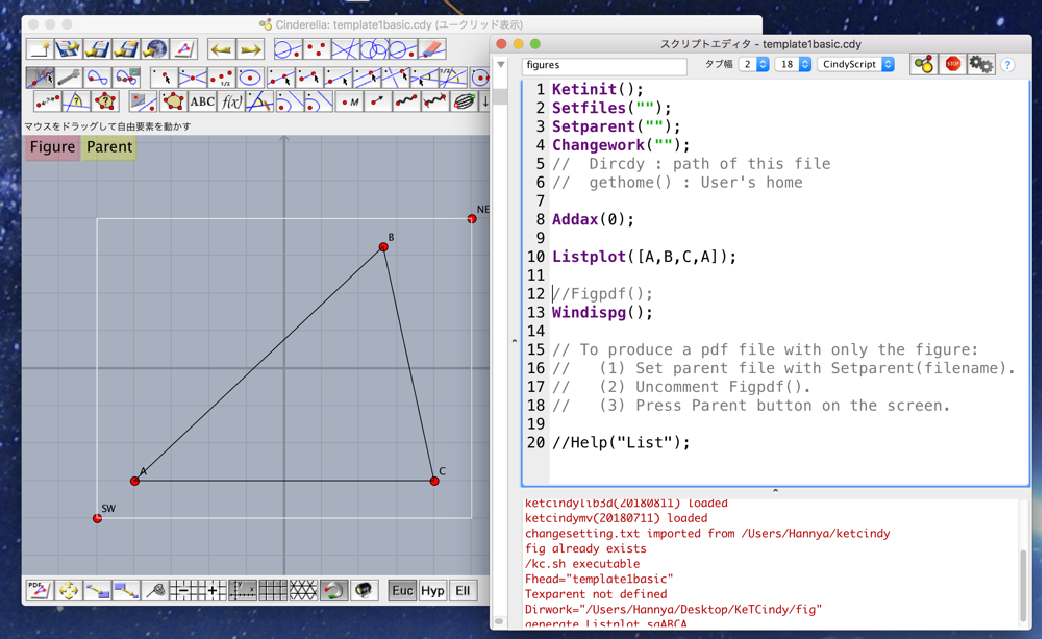
\includegraphics[bb=0.00 0.00 500.03 306.52,width=10cm]{Fig/start01.pdf}\end{center}

この三角形で Cinderellaの作図機能を用いて内心を求め,内接円を描く。

まず,スクリプトエディタの \verb|Listplot([A,B,C,A]);|  の行頭にスラッシュを2本書き入れ,Shift+Enter で実行する。こうすると,この行はコメント行となり実行されない行になる。その結果,三角形が消えて点だけ残る。

画面上部の作図ツールから「線分を加える」
\includegraphics[bb=0.00 0.00 6.48 5.04,width=8mm]{Fig/segment.pdf} をクリックして選択し,点Aから点Bへドラッグすると線分が描かれる。同様にして,BC, CAを引く。

\begin{center}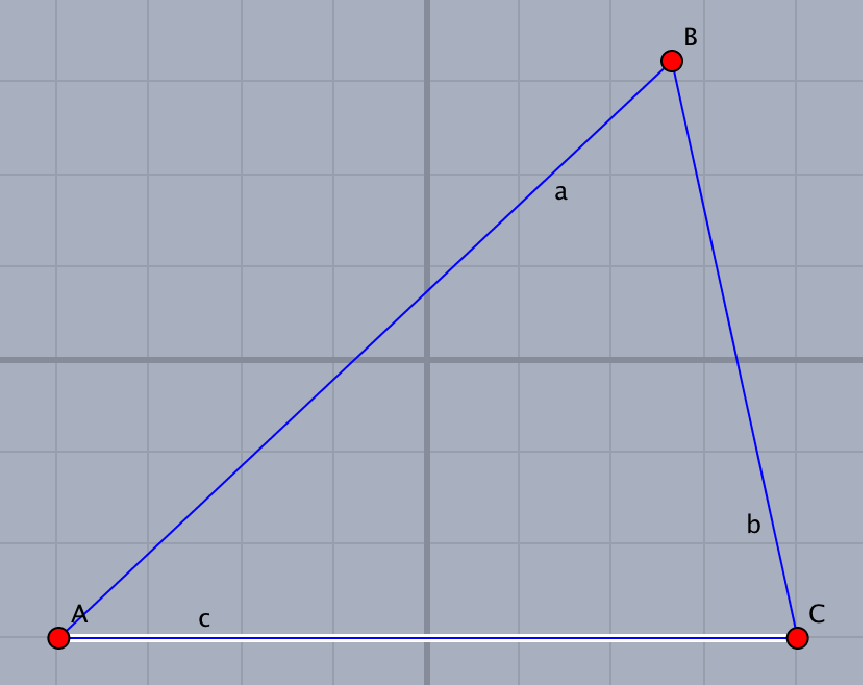
\includegraphics[bb=0.00 0.00 414.02 329.02,height=3.5cm]{Fig/start02.pdf} \end{center}

次に,角の二等分線を引く。「角の二等分線を加える」ツール 
\includegraphics[bb=0.00 0.00 6.48 5.04,width=8mm]{Fig/bisector.pdf} を選択し,辺BA,BCを順にクリックすると角ABCの二等分線が引かれる。 このとき,次図左のように,該当する角を表すガイドが出る。

\hspace{20mm}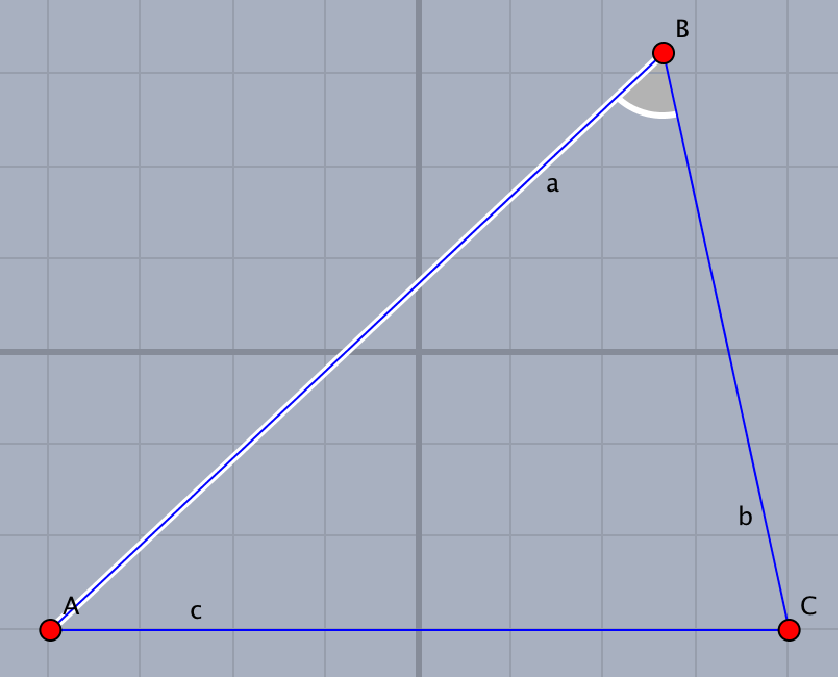
\includegraphics[bb=0.00 0.00 402.02 325.02,height=3cm]{Fig/start03.pdf} \hspace{5mm}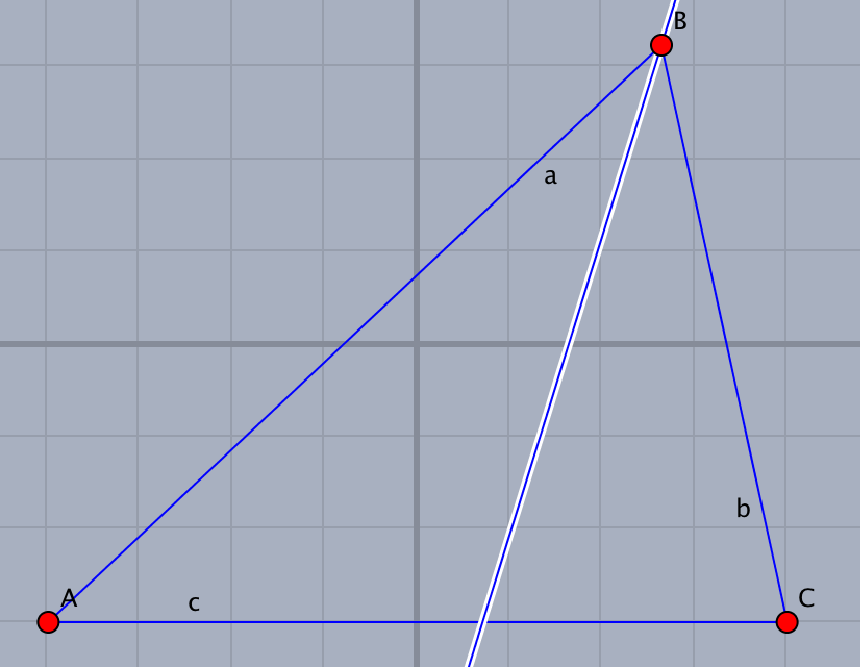
\includegraphics[bb=0.00 0.00 413.02 320.02,height=3cm]{Fig/start04.pdf}

同様にして,角Aの二等分線を引き,「交点を求める」ツール
\includegraphics[bb=0.00 0.00 6.48 5.04,width=8mm]{Fig/intersection.pdf}をクリックして,2本の二等分線を順にクリックすると交点が求められる。(角Aの二等分線を引いた直後はこれが選択状態にあるので,角Bの二等分線をクリックすればよい)

\begin{center}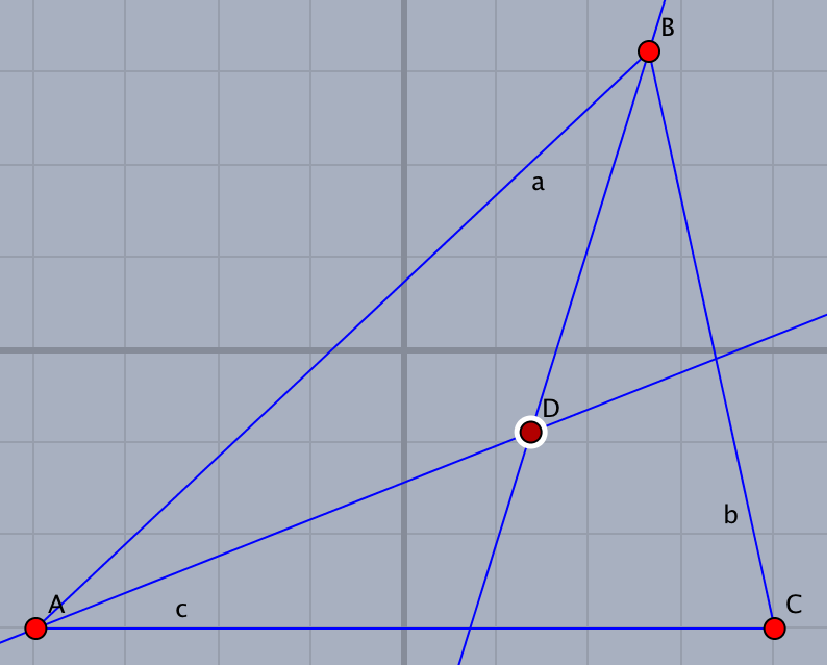
\includegraphics[bb=0.00 0.00 397.02 319.02,height=3cm]{Fig/start05.pdf}\end{center}

内接円の半径を決めるために,辺ACに垂直で点Dを通る直線を描く。「垂線を加える」ツール 
\includegraphics[bb=0.00 0.00 6.48 5.04,width=8mm]{Fig/multi-add-perp.pdf} を選択し,辺AC上でマウスボタンを押し,そのまま点Dへドラッグすると垂線が引ける。

\hspace{20mm}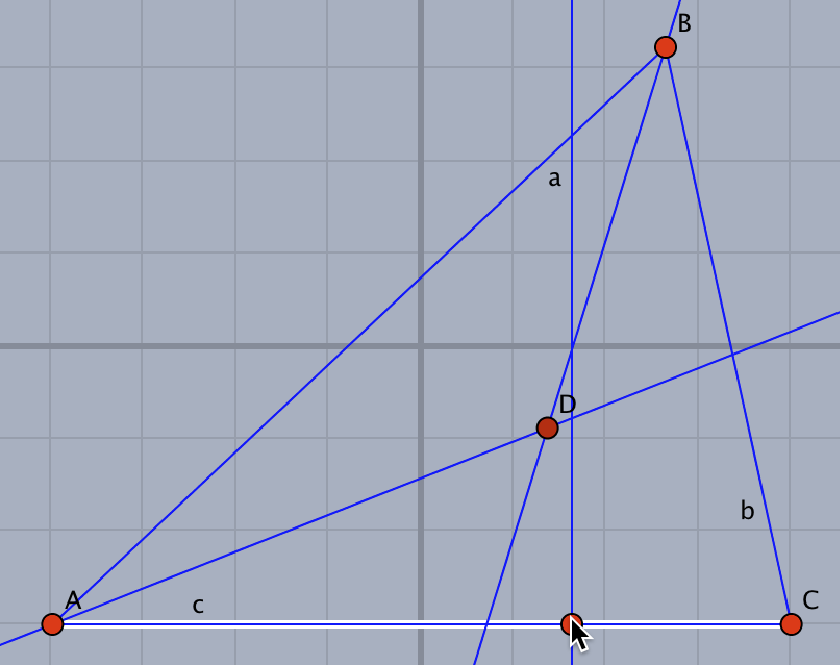
\includegraphics[bb=0.00 0.00 403.02 319.02,height=3cm]{Fig/start06.pdf} \hspace{5mm}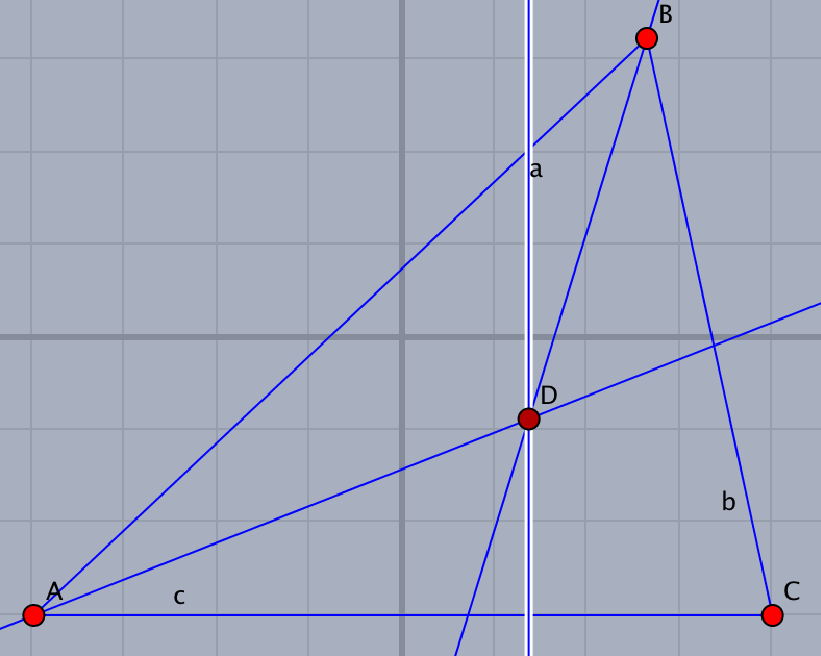
\includegraphics[bb=0.00 0.00 394.02 315.02,height=3cm]{Fig/start07.pdf} 

最後に,垂線と辺ACの交点を求める。

\begin{center}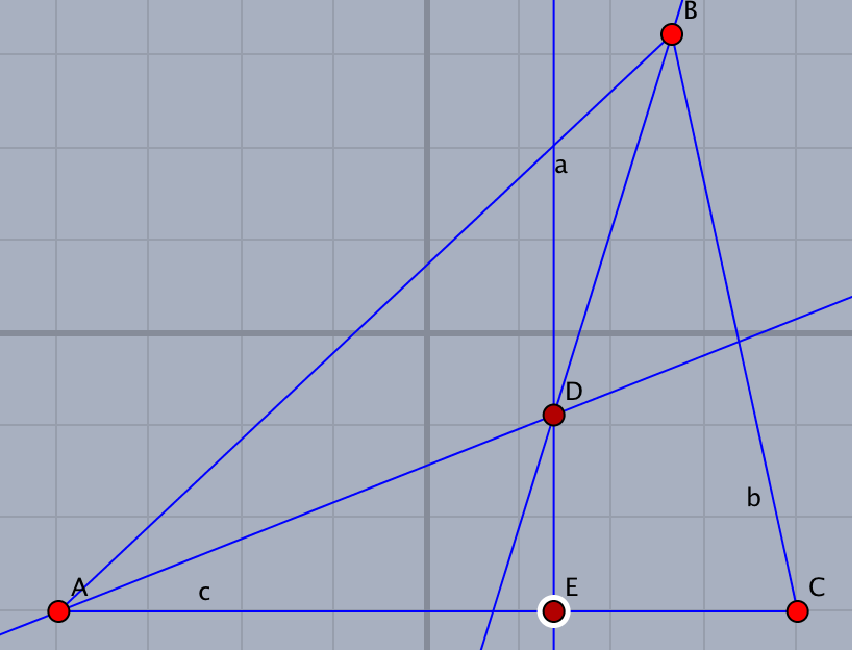
\includegraphics[bb=0.00 0.00 409.02 312.02,height=3cm]{Fig/start08.pdf}\end{center}

図が描かれたら,「要素を動かす」ツール 
\includegraphics[bb=0.00 0.00 6.48 5.04,width=8mm]{Fig/move.pdf} を選択して,始めの状態(動かすモード)に戻しておく。

これで内心の作図と半径の作図ができた。内心円は描かなくてよい。

スクリプトエディタに戻り,先ほど書いた // を消して \verb|Listplot([A,B,C,A]);|  を有効にし,次のスクリプトを追加し,Shift+Enterで実行すると,内接円が描かれる。なお,2行目を \verb|Setfiles("innercircle")| として,ファイル名も設定しておく。

\begin{verbatim}
    Circledata([D,E]);
    Pointdata("1",[D],["size=3"]);
    Letter([A,"sw","A",B,"ne","B",C,"se","C",D,"ne2","I"]);
\end{verbatim}

\begin{center}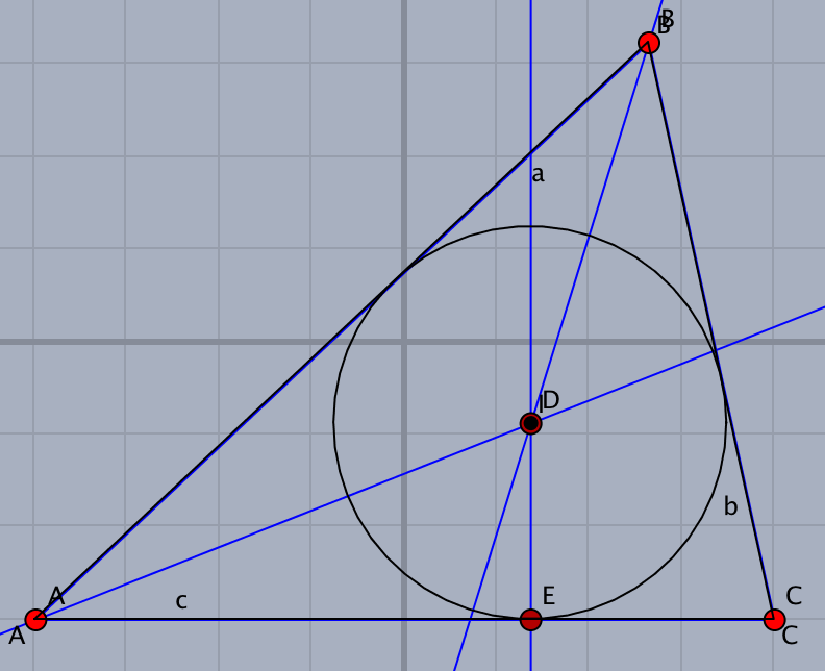
\includegraphics[bb=0.00 0.00 396.02 322.02,height=4cm]{Fig/start09.pdf} \end{center}


画面左上の「Figure」ボタンをクリックすると,プレビュー用のPDFができて表示される(下図左)。
描画面で点Bをドラッグして三角形の形を変えれば,それに応じて出力する図も変えることができる(下図右)。

\begin{center} 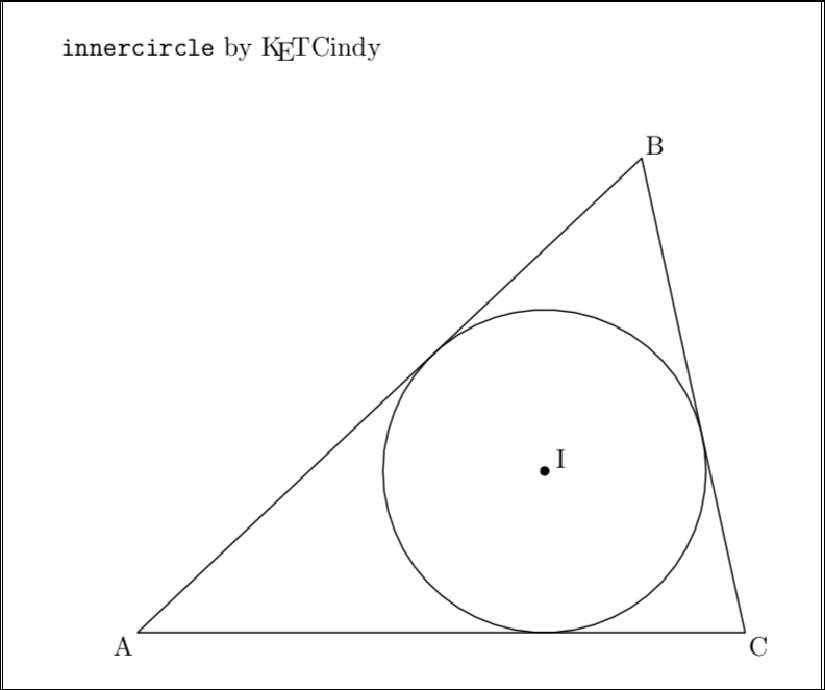
\includegraphics[bb=0.00 0.00 396.02 331.02,height=4cm]{Fig/start10.pdf}  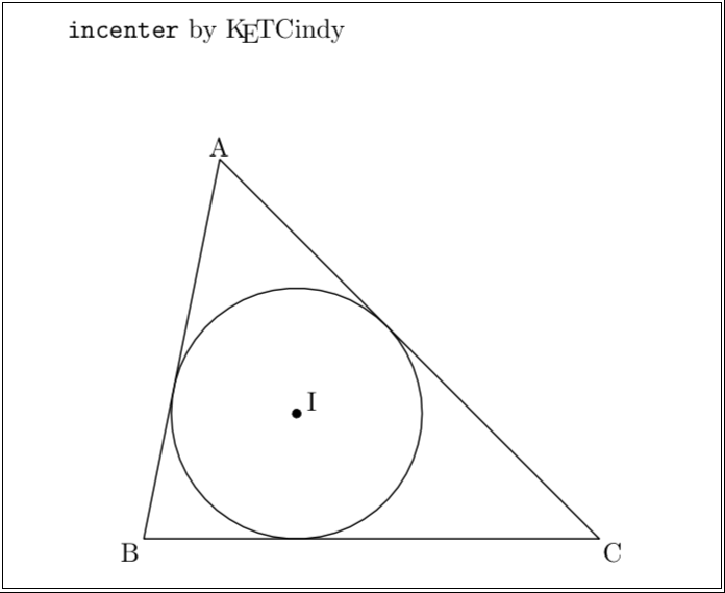
\includegraphics[bb=0.00 0.00 348.02 284.51,height=4cm]{Fig/incenter03.pdf} \end{center}

\vspace{\baselineskip}
\ketcindy がTikZなどの作図支援ツールと異なるのは,Cinderellaの作図機能を用いてインタラクティブに図の調整ができる点である。簡単な図であれば,座標の計算は不要で,Cinderellaの作図画面を見ながら\ketcindy の作図関数でプログラムを書くだけでよい。

なお,Cinderellaの作図機能については,付録の \hyperlink{geometrytool}{作図ツール} を参照されたい。

%---------------- 関数のグラフ--------------------------
\subsubsection{関数のグラフ}

例として,$y=\sin x$ と $y=x$  のグラフを描く。

template.cdy をダブルクリックして開き,Ctrl+9 ( Windows ) /  ⌘+9 ( Mac ) でスクリプトエディタを開く。

座標軸を描くので,\verb|Addax(0);| を \verb|Addax(1);| に変え,\verb|Listplot([A,B,C,A]);| は使わないので削除し,かわりに次のスクリプトを書く。

\begin{layer}{150}{0}
\putnotese{80}{5}{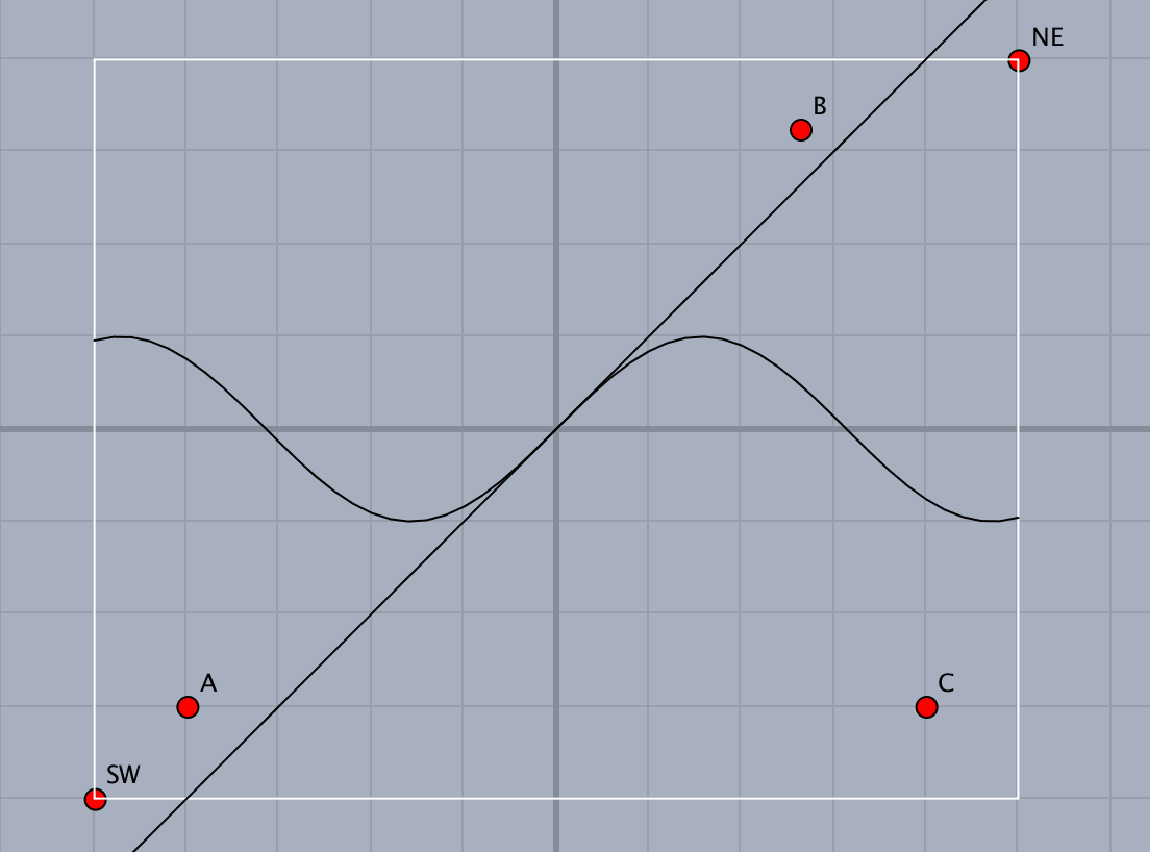
\includegraphics[bb=0.00 0.00 552.03 409.02,height=30mm]{Fig/xsinx01.pdf} }
\end{layer}
\begin{verbatim}
    Plotdata("1","y=sin(x)","x");
    Plotdata("2","y=x","x");
\end{verbatim}

これだけで右のようにグラフが描かれる。

\vspace{15mm}
%\begin{center}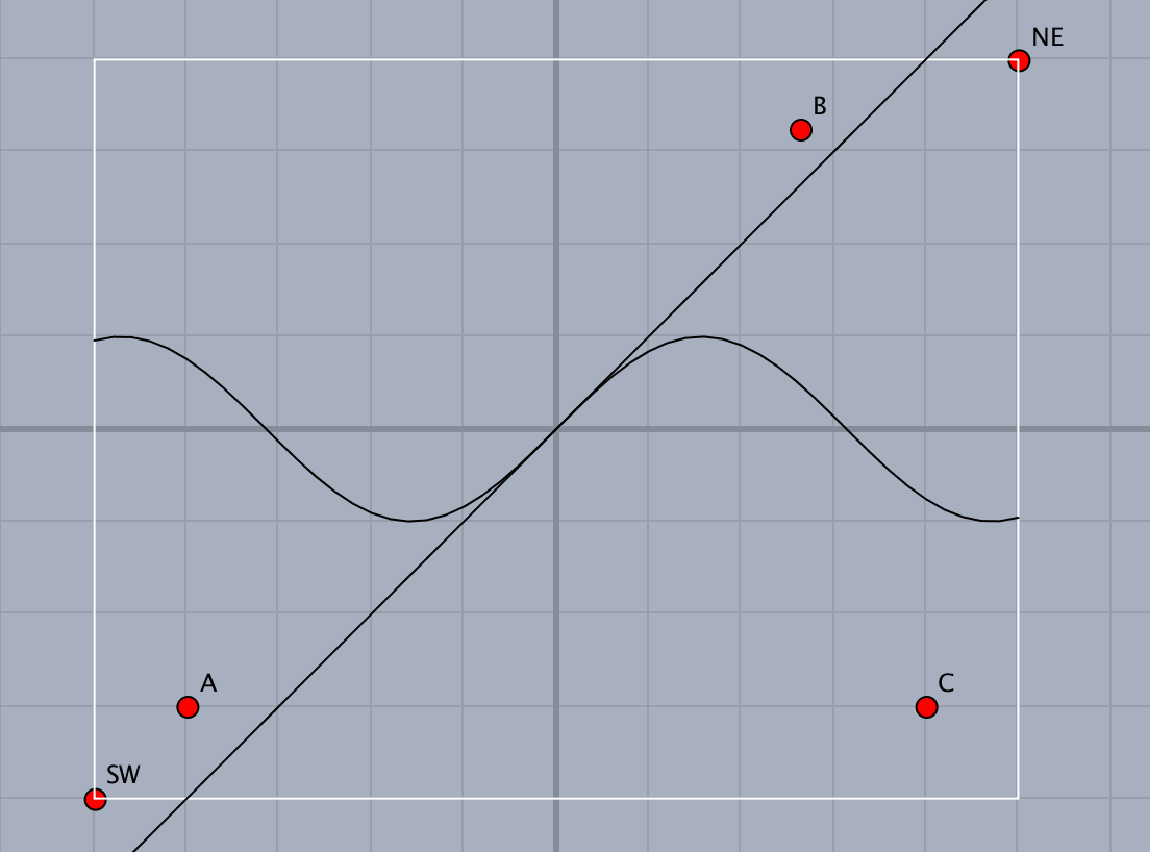
\includegraphics[bb=0.00 0.00 552.03 409.02,height=30mm]{Fig/xsinx01.pdf} \end{center}

描画範囲は点NEとSWをドラッグして適当に決めよう。また,点A,B,Cが残ったままだが,これを関数名を表示する場所として利用するために適当な位置にドラッグして移動する。

\begin{center}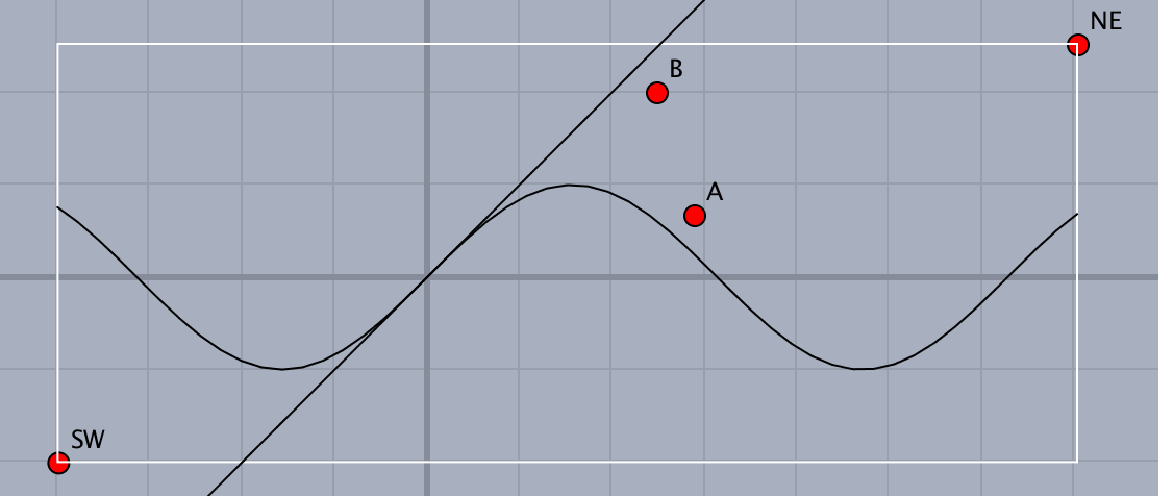
\includegraphics[bb=0.00 0.00 556.03 238.01,height=30mm]{Fig/xsinx02.pdf} \end{center}

関数名と$x$軸上の交点を表示するために,関数 \verb|Expr()| を使って次のように書く。
\begin{verbatim}
    Expr([A,"e","y=\sin x",B,"e","y=x",[-pi,0],"s2","-\pi",[pi,0],"s2","\pi",
    [2*pi,0],"s2","2\pi"]);
\end{verbatim}

注)改行せず1行に書いてよい。

\begin{center}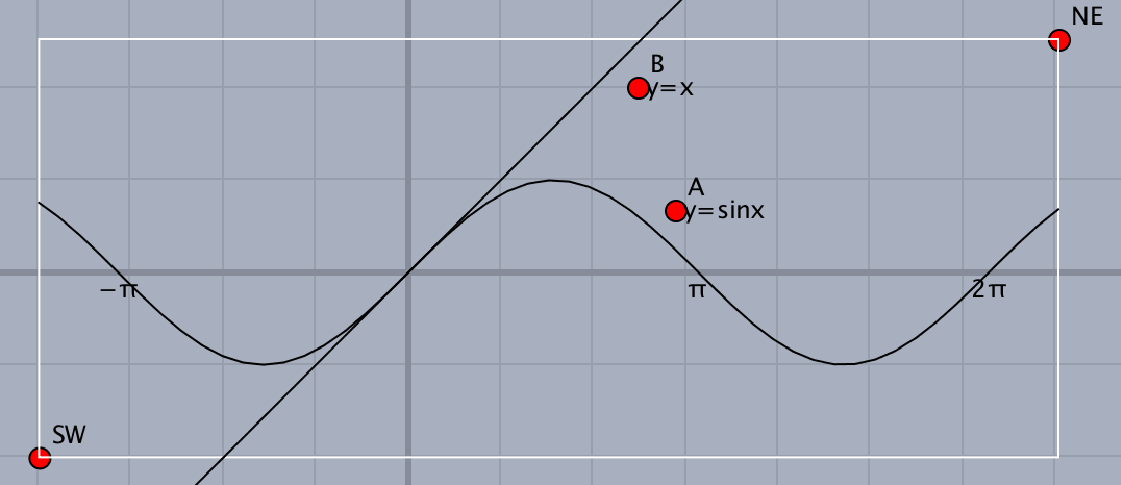
\includegraphics[bb=0.00 0.00 546.03 236.01,height=30mm]{Fig/xsinx03.pdf} \end{center}

\verb|Figure| ボタンをクリックすると,次の図が描かれる。

\vspace{\baselineskip}
\begin{center}%%% /Users/Hannya/Desktop/KeTCindy/fig/xsinx.tex 
%%% Generator=template1basic.cdy 
{\unitlength=7mm%
\begin{picture}%
(11.04,4.53)(-4,-2)%
\special{pn 8}%
%
{%
\color[rgb]{0,0,0}%
\special{pa -1102  -209}\special{pa -1042  -164}\special{pa  -981  -112}\special{pa  -920   -54}%
\special{pa  -859     7}\special{pa  -798    67}\special{pa  -737   124}\special{pa  -676   175}%
\special{pa  -616   217}\special{pa  -555   249}\special{pa  -494   269}\special{pa  -433   276}%
\special{pa  -372   269}\special{pa  -311   249}\special{pa  -250   217}\special{pa  -190   175}%
\special{pa  -129   124}\special{pa   -68    67}\special{pa    -7     7}\special{pa    54   -53}%
\special{pa   115  -111}\special{pa   175  -164}\special{pa   236  -208}\special{pa   297  -243}%
\special{pa   358  -265}\special{pa   419  -275}\special{pa   480  -272}\special{pa   541  -255}%
\special{pa   601  -226}\special{pa   662  -186}\special{pa   723  -136}\special{pa   784   -81}%
\special{pa   845   -21}\special{pa   906    40}\special{pa   967    99}\special{pa  1027   153}%
\special{pa  1088   199}\special{pa  1149   236}\special{pa  1210   261}\special{pa  1271   274}%
\special{pa  1332   274}\special{pa  1393   260}\special{pa  1453   233}\special{pa  1514   196}%
\special{pa  1575   148}\special{pa  1636    94}\special{pa  1697    35}\special{pa  1758   -26}%
\special{pa  1818   -85}\special{pa  1879  -141}\special{pa  1940  -189}%
\special{fp}%
}%
{%
\color[rgb]{0,0,0}%
\special{pa  -551   551}\special{pa  -494   494}\special{pa  -433   433}\special{pa  -372   372}%
\special{pa  -311   311}\special{pa  -250   250}\special{pa  -190   190}\special{pa  -129   129}%
\special{pa   -68    68}\special{pa    -7     7}\special{pa    54   -54}\special{pa   115  -115}%
\special{pa   175  -175}\special{pa   236  -236}\special{pa   297  -297}\special{pa   358  -358}%
\special{pa   419  -419}\special{pa   480  -480}\special{pa   541  -541}\special{pa   601  -601}%
\special{pa   662  -662}\special{pa   697  -697}%
\special{fp}%
}%
{%
\color[rgb]{0,0,0}%
\settowidth{\Width}{$y=\sin x$}\setlength{\Width}{0\Width}%
\settoheight{\Height}{$y=\sin x$}\settodepth{\Depth}{$y=\sin x$}\setlength{\Height}{-0.5\Height}\setlength{\Depth}{0.5\Depth}\addtolength{\Height}{\Depth}%
\put(2.9614286,0.6800000){\hspace*{\Width}\raisebox{\Height}{$y=\sin x$}}%
%
}%
{%
\color[rgb]{0,0,0}%
\settowidth{\Width}{$y=x$}\setlength{\Width}{0\Width}%
\settoheight{\Height}{$y=x$}\settodepth{\Depth}{$y=x$}\setlength{\Height}{-0.5\Height}\setlength{\Depth}{0.5\Depth}\addtolength{\Height}{\Depth}%
\put(2.5514286,2.0100000){\hspace*{\Width}\raisebox{\Height}{$y=x$}}%
%
}%
{%
\color[rgb]{0,0,0}%
\settowidth{\Width}{$-\pi$}\setlength{\Width}{-0.5\Width}%
\settoheight{\Height}{$-\pi$}\settodepth{\Depth}{$-\pi$}\setlength{\Height}{-\Height}%
\put(-3.1400000,-0.2142857){\hspace*{\Width}\raisebox{\Height}{$-\pi$}}%
%
}%
{%
\color[rgb]{0,0,0}%
\settowidth{\Width}{$\pi$}\setlength{\Width}{-0.5\Width}%
\settoheight{\Height}{$\pi$}\settodepth{\Depth}{$\pi$}\setlength{\Height}{-\Height}%
\put(3.1400000,-0.2142857){\hspace*{\Width}\raisebox{\Height}{$\pi$}}%
%
}%
{%
\color[rgb]{0,0,0}%
\settowidth{\Width}{$2\pi$}\setlength{\Width}{-0.5\Width}%
\settoheight{\Height}{$2\pi$}\settodepth{\Depth}{$2\pi$}\setlength{\Height}{-\Height}%
\put(6.2800000,-0.2142857){\hspace*{\Width}\raisebox{\Height}{$2\pi$}}%
%
}%
\special{pa -1102    -0}\special{pa  1940    -0}%
\special{fp}%
\special{pa     0   551}\special{pa     0  -697}%
\special{fp}%
\settowidth{\Width}{$x$}\setlength{\Width}{0\Width}%
\settoheight{\Height}{$x$}\settodepth{\Depth}{$x$}\setlength{\Height}{-0.5\Height}\setlength{\Depth}{0.5\Depth}\addtolength{\Height}{\Depth}%
\put(7.1114286,0.0000000){\hspace*{\Width}\raisebox{\Height}{$x$}}%
%
\settowidth{\Width}{$y$}\setlength{\Width}{-0.5\Width}%
\settoheight{\Height}{$y$}\settodepth{\Depth}{$y$}\setlength{\Height}{\Depth}%
\put(0.0000000,2.6014286){\hspace*{\Width}\raisebox{\Height}{$y$}}%
%
\settowidth{\Width}{O}\setlength{\Width}{-1\Width}%
\settoheight{\Height}{O}\settodepth{\Depth}{O}\setlength{\Height}{-\Height}%
\put(-0.0714286,-0.0714286){\hspace*{\Width}\raisebox{\Height}{O}}%
%
\end{picture}}% \end{center}


%----------------  空間図形 --------------------------
\subsubsection{空間図形}

\ketcindy のシステムに同梱されている samples フォルダから,s05spacefigure フォルダを開き,s0501basic.cdy をひな形として使う。適当な場所に複製を作り,名前を変えておくとよい。ここでは,3Dbasic.cdy として進める。

3Dbasic.cdy を開くと次のような画面になる。

\vspace{\baselineskip}
\begin{center}
 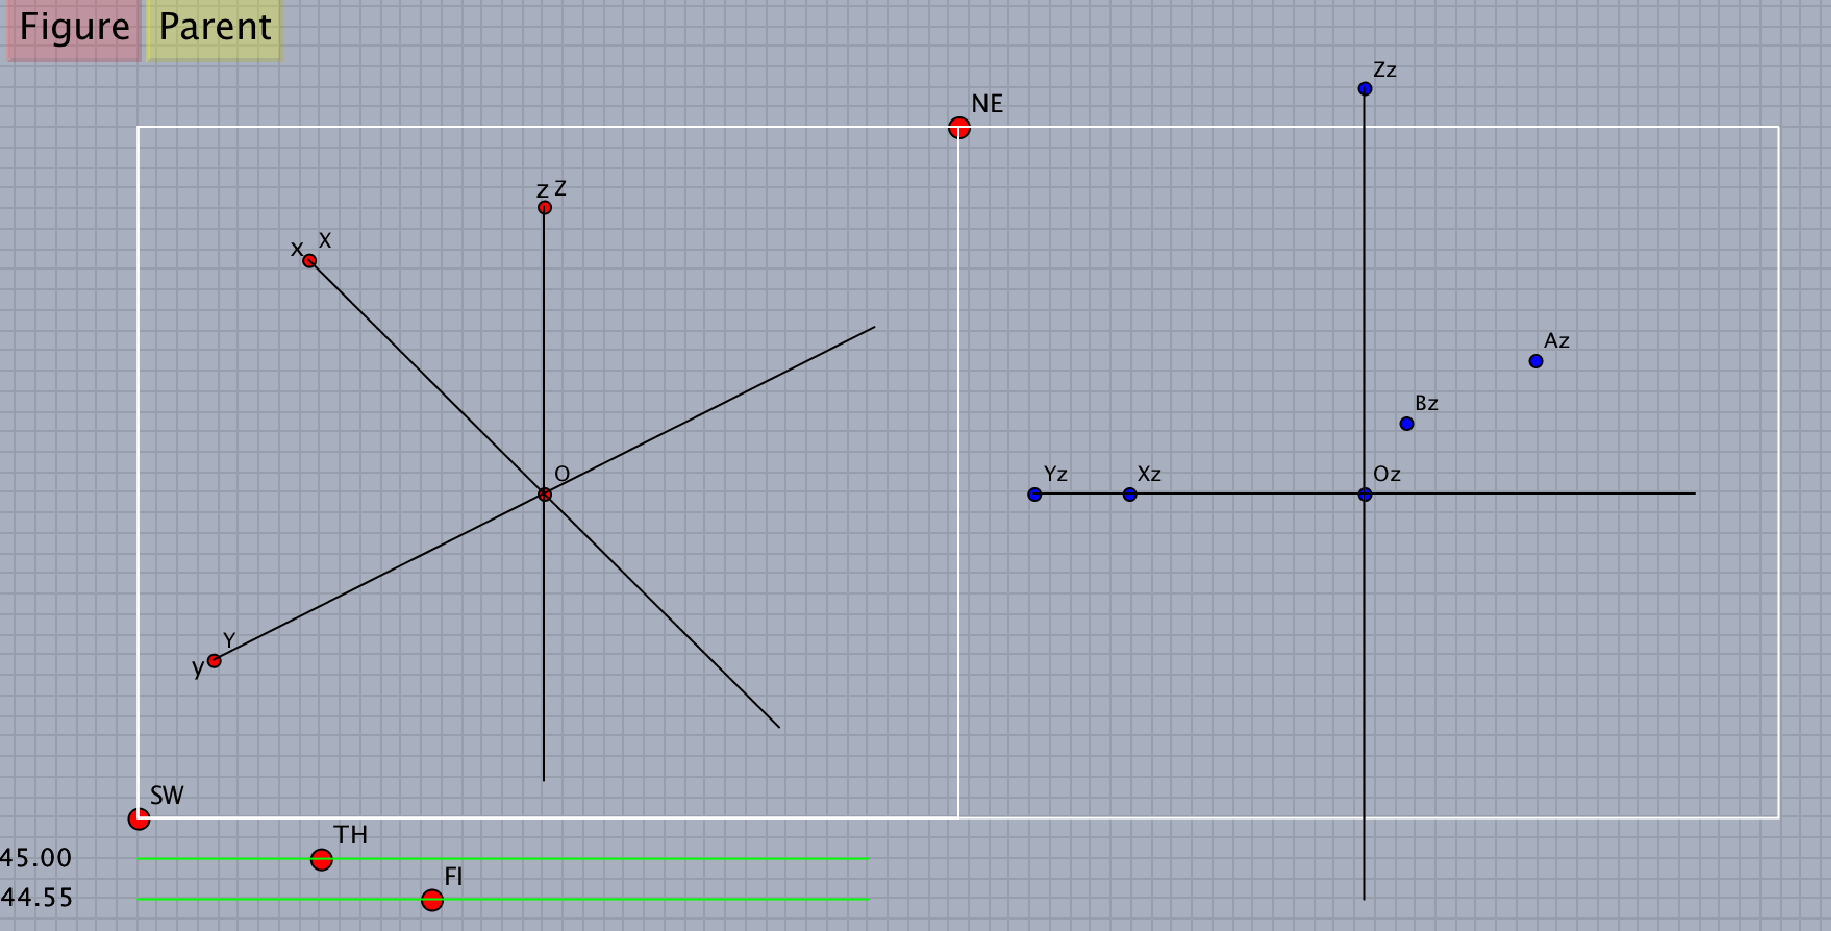
\includegraphics[bb=0 0 879.05 447.02 , width=8cm]{Fig/3dstart.pdf}
\end{center}

下のスライダで点TH,Fl をドラッグすると,空間での視点の位置が変わる。(座標軸が回転する)

ここでは,正四面体と,高さを求めるのによく使われる補助線を描いてみよう。スクリプトエディタを開き,次の3行を消す。

\begin{verbatim}
    Ch=[1];
    if(contains(Ch,1),
     Skeletonparadata("1",[1.5]);
    );
\end{verbatim}

かわりに次のスクリプトを書いて Shift+Enter で実行する。

\begin{layer}{150}{0}
\putnotese{90}{0}{ %%% /Users/Hannya/Desktop/KeTCindy/fig/tetrahedron.tex 
%%% Generator=3Dbasic.cdy 
{\unitlength=1cm%
\begin{picture}%
(5,4.65)(-2.54,-0.95)%
\special{pn 8}%
%
{%
\color[rgb]{0,0,0}%
}%
{%
\color[rgb]{0,0,0}%
}%
{%
\color[rgb]{0,0,0}%
}%
{%
\color[rgb]{0,0,0}%
}%
{%
\color[rgb]{0,0,0}%
}%
{%
\color[rgb]{0,0,0}%
}%
{%
\color[rgb]{0,0,0}%
}%
{%
\color[rgb]{0,0,0}%
}%
{%
\color[rgb]{0,0,0}%
}%
{%
\color[rgb]{0,0,0}%
}%
{%
\color[rgb]{0,0,0}%
\special{pn 8}%
\special{pa 767 -155}\special{pa 759 -155}\special{fp}\special{pa 728 -154}\special{pa 720 -154}\special{fp}%
\special{pa 688 -154}\special{pa 680 -153}\special{fp}\special{pa 649 -153}\special{pa 641 -153}\special{fp}%
\special{pa 610 -152}\special{pa 602 -152}\special{fp}\special{pa 570 -152}\special{pa 562 -152}\special{fp}%
\special{pa 531 -151}\special{pa 523 -151}\special{fp}\special{pa 492 -150}\special{pa 484 -150}\special{fp}%
\special{pa 452 -150}\special{pa 444 -150}\special{fp}\special{pa 413 -149}\special{pa 405 -149}\special{fp}%
\special{pa 374 -148}\special{pa 366 -148}\special{fp}\special{pa 334 -148}\special{pa 326 -148}\special{fp}%
\special{pa 295 -147}\special{pa 287 -147}\special{fp}\special{pa 256 -147}\special{pa 248 -146}\special{fp}%
\special{pa 217 -146}\special{pa 209 -146}\special{fp}\special{pa 177 -145}\special{pa 169 -145}\special{fp}%
\special{pa 138 -145}\special{pa 130 -145}\special{fp}\special{pa 99 -144}\special{pa 91 -144}\special{fp}%
\special{pa 59 -143}\special{pa 51 -143}\special{fp}\special{pa 20 -143}\special{pa 12 -143}\special{fp}%
\special{pa -19 -142}\special{pa -27 -142}\special{fp}\special{pa -59 -142}\special{pa -67 -141}\special{fp}%
\special{pa -98 -141}\special{pa -106 -141}\special{fp}\special{pa -137 -140}\special{pa -145 -140}\special{fp}%
\special{pa -177 -140}\special{pa -185 -139}\special{fp}\special{pa -216 -139}\special{pa -224 -139}\special{fp}%
\special{pa -255 -138}\special{pa -263 -138}\special{fp}\special{pa -295 -138}\special{pa -303 -138}\special{fp}%
\special{pa -334 -137}\special{pa -342 -137}\special{fp}\special{pa -373 -136}\special{pa -381 -136}\special{fp}%
\special{pa -413 -136}\special{pa -421 -136}\special{fp}\special{pa -452 -135}\special{pa -460 -135}\special{fp}%
\special{pa -491 -135}\special{pa -499 -134}\special{fp}\special{pa -531 -134}\special{pa -539 -134}\special{fp}%
\special{pa -570 -133}\special{pa -578 -133}\special{fp}\special{pa -609 -133}\special{pa -617 -133}\special{fp}%
\special{pa -648 -132}\special{pa -656 -132}\special{fp}\special{pa -688 -131}\special{pa -696 -131}\special{fp}%
\special{pa -727 -131}\special{pa -735 -131}\special{fp}\special{pa -766 -130}\special{pa -774 -130}\special{fp}%
\special{pa -806 -129}\special{pa -814 -129}\special{fp}\special{pn 8}%
}%
{%
\color[rgb]{0,0,0}%
\special{pa     0 -1294}\special{pa  -381    77}%
\special{fp}%
}%
{%
\color[rgb]{0,0,0}%
\special{pn 8}%
\special{pa -385 78}\special{pa -378 77}\special{fp}\special{pa -347 71}\special{pa -339 69}\special{fp}%
\special{pa -309 63}\special{pa -301 61}\special{fp}\special{pa -271 55}\special{pa -263 54}\special{fp}%
\special{pa -233 48}\special{pa -225 46}\special{fp}\special{pa -195 40}\special{pa -187 38}\special{fp}%
\special{pa -156 32}\special{pa -149 31}\special{fp}\special{pa -118 24}\special{pa -110 23}\special{fp}%
\special{pa -80 17}\special{pa -72 15}\special{fp}\special{pa -42 9}\special{pa -34 7}\special{fp}%
\special{pa -4 1}\special{pa 4 0}\special{fp}\special{pa 34 -7}\special{pa 42 -8}\special{fp}%
\special{pa 72 -14}\special{pa 80 -16}\special{fp}\special{pa 111 -22}\special{pa 118 -24}\special{fp}%
\special{pa 149 -30}\special{pa 157 -31}\special{fp}\special{pa 187 -37}\special{pa 195 -39}\special{fp}%
\special{pa 225 -45}\special{pa 233 -47}\special{fp}\special{pa 263 -53}\special{pa 271 -54}\special{fp}%
\special{pa 301 -61}\special{pa 309 -62}\special{fp}\special{pa 339 -68}\special{pa 347 -70}\special{fp}%
\special{pa 378 -76}\special{pa 385 -78}\special{fp}\special{pa 416 -84}\special{pa 424 -85}\special{fp}%
\special{pa 454 -92}\special{pa 462 -93}\special{fp}\special{pa 492 -99}\special{pa 500 -101}\special{fp}%
\special{pa 530 -107}\special{pa 538 -109}\special{fp}\special{pa 568 -115}\special{pa 576 -116}\special{fp}%
\special{pa 607 -122}\special{pa 614 -124}\special{fp}\special{pa 645 -130}\special{pa 653 -132}\special{fp}%
\special{pa 683 -138}\special{pa 691 -140}\special{fp}\special{pa 721 -146}\special{pa 729 -147}\special{fp}%
\special{pa 759 -153}\special{pa 767 -155}\special{fp}\special{pn 8}%
}%
{%
\color[rgb]{0,0,0}%
\special{pn 8}%
\special{pa 767 -155}\special{pa 759 -155}\special{fp}\special{pa 728 -154}\special{pa 720 -154}\special{fp}%
\special{pa 688 -154}\special{pa 680 -153}\special{fp}\special{pa 649 -153}\special{pa 641 -153}\special{fp}%
\special{pa 610 -152}\special{pa 602 -152}\special{fp}\special{pa 570 -152}\special{pa 562 -152}\special{fp}%
\special{pa 531 -151}\special{pa 523 -151}\special{fp}\special{pa 492 -150}\special{pa 484 -150}\special{fp}%
\special{pa 452 -150}\special{pa 444 -150}\special{fp}\special{pa 413 -149}\special{pa 405 -149}\special{fp}%
\special{pa 374 -148}\special{pa 366 -148}\special{fp}\special{pa 334 -148}\special{pa 326 -148}\special{fp}%
\special{pa 295 -147}\special{pa 287 -147}\special{fp}\special{pa 256 -147}\special{pa 248 -146}\special{fp}%
\special{pa 217 -146}\special{pa 209 -146}\special{fp}\special{pa 177 -145}\special{pa 169 -145}\special{fp}%
\special{pa 138 -145}\special{pa 130 -145}\special{fp}\special{pa 99 -144}\special{pa 91 -144}\special{fp}%
\special{pa 59 -143}\special{pa 51 -143}\special{fp}\special{pa 20 -143}\special{pa 12 -143}\special{fp}%
\special{pa -19 -142}\special{pa -27 -142}\special{fp}\special{pa -59 -142}\special{pa -67 -141}\special{fp}%
\special{pa -98 -141}\special{pa -106 -141}\special{fp}\special{pa -137 -140}\special{pa -145 -140}\special{fp}%
\special{pa -177 -140}\special{pa -185 -139}\special{fp}\special{pa -216 -139}\special{pa -224 -139}\special{fp}%
\special{pa -255 -138}\special{pa -263 -138}\special{fp}\special{pa -295 -138}\special{pa -303 -138}\special{fp}%
\special{pa -334 -137}\special{pa -342 -137}\special{fp}\special{pa -373 -136}\special{pa -381 -136}\special{fp}%
\special{pa -413 -136}\special{pa -421 -136}\special{fp}\special{pa -452 -135}\special{pa -460 -135}\special{fp}%
\special{pa -491 -135}\special{pa -499 -134}\special{fp}\special{pa -531 -134}\special{pa -539 -134}\special{fp}%
\special{pa -570 -133}\special{pa -578 -133}\special{fp}\special{pa -609 -133}\special{pa -617 -133}\special{fp}%
\special{pa -648 -132}\special{pa -656 -132}\special{fp}\special{pa -688 -131}\special{pa -696 -131}\special{fp}%
\special{pa -727 -131}\special{pa -735 -131}\special{fp}\special{pa -766 -130}\special{pa -774 -130}\special{fp}%
\special{pa -806 -129}\special{pa -814 -129}\special{fp}\special{pn 8}%
}%
{%
\color[rgb]{0,0,0}%
\special{pa  -810  -129}\special{pa    47   284}%
\special{fp}%
}%
{%
\color[rgb]{0,0,0}%
\special{pa   763  -155}\special{pa    47   284}%
\special{fp}%
}%
{%
\color[rgb]{0,0,0}%
\special{pa  -810  -129}\special{pa     0 -1295}%
\special{fp}%
}%
{%
\color[rgb]{0,0,0}%
\special{pa   763  -155}\special{pa     0 -1295}%
\special{fp}%
}%
{%
\color[rgb]{0,0,0}%
\special{pa    47   284}\special{pa     0 -1295}%
\special{fp}%
}%
\end{picture}}%}
\end{layer}
\begin{verbatim}
   Putpoint3d("A",2*[-1,-1/sqrt(3),0],"fix");
   Putpoint3d("B",2*[1,-1/sqrt(3),0],"fix");
   Putpoint3d("C",2*[0,sqrt(3)-1/sqrt(3),0],"fix");
   Putpoint3d("D",2*[0,0,sqrt(3)],"fix");
   Putpoint3d("M",(B3d+C3d)/2,"fix");
   phd=Concatobj([[A,B,C],[A,B,D],[A,C,D],[B,C,D]]);
   Spaceline("1",[D,M,A]);
   VertexEdgeFace("1",phd,["Edg=nogeo"]);
   Nohiddenbyfaces("1","phf3d1");
\end{verbatim}


%----------------  作表 --------------------------
\subsubsection{作表}

\TeX\ で表を作るのはかなり面倒だが,\ketcindy\ を使えば比較的簡単に作表ができる。次の図は関数の増減・凹凸表である。以下は紹介にとどめる。関数リファレンスに例を掲載しているので参照されたい。

\begin{center} %%% /Users/Hannya/ketcindy/ketwork/zogen3.tex 2016-12-8 15:42
%%% zogen3.sce 2016-12-8 15:42
{\unitlength=1cm%
\begin{picture}%
(   8.00000,   4.00000)(  -0.00000,  -0.00000)%
\special{pn 8}%
%
\special{pa 0 -1575}\special{pa 0 0}%
\special{fp}%
\special{pa 394 -1575}\special{pa 394 0}%
\special{fp}%
\special{pa 787 -1575}\special{pa 787 0}%
\special{fp}%
\special{pa 1181 -1575}\special{pa 1181 0}%
\special{fp}%
\special{pa 1575 -1575}\special{pa 1575 0}%
\special{fp}%
\special{pa 1969 -1575}\special{pa 1969 0}%
\special{fp}%
\special{pa 2362 -1575}\special{pa 2362 0}%
\special{fp}%
\special{pa 2756 -1575}\special{pa 2756 0}%
\special{fp}%
\special{pa 3150 -1575}\special{pa 3150 0}%
\special{fp}%
\special{pa 0 -1575}\special{pa 3150 -1575}%
\special{fp}%
\special{pa 0 -1181}\special{pa 3150 -1181}%
\special{fp}%
\special{pa 0 -787}\special{pa 3150 -787}%
\special{fp}%
\special{pa 0 -394}\special{pa 3150 -394}%
\special{fp}%
\special{pa 0 0}\special{pa 3150 0}%
\special{fp}%
\settowidth{\Width}{$x$}\setlength{\Width}{-0.5\Width}%
\settoheight{\Height}{$x$}\settodepth{\Depth}{$x$}\setlength{\Height}{-0.5\Height}\setlength{\Depth}{0.5\Depth}\addtolength{\Height}{\Depth}%
\put(0.5000,3.5000){\hspace*{\Width}\raisebox{\Height}{$x$}}%
%
%
\settowidth{\Width}{$\cdots$}\setlength{\Width}{-0.5\Width}%
\settoheight{\Height}{$\cdots$}\settodepth{\Depth}{$\cdots$}\setlength{\Height}{-0.5\Height}\setlength{\Depth}{0.5\Depth}\addtolength{\Height}{\Depth}%
\put(1.5000,3.5000){\hspace*{\Width}\raisebox{\Height}{$\cdots$}}%
%
%
\settowidth{\Width}{$-1$}\setlength{\Width}{-0.5\Width}%
\settoheight{\Height}{$-1$}\settodepth{\Depth}{$-1$}\setlength{\Height}{-0.5\Height}\setlength{\Depth}{0.5\Depth}\addtolength{\Height}{\Depth}%
\put(2.5000,3.5000){\hspace*{\Width}\raisebox{\Height}{$-1$}}%
%
%
\settowidth{\Width}{$\cdots$}\setlength{\Width}{-0.5\Width}%
\settoheight{\Height}{$\cdots$}\settodepth{\Depth}{$\cdots$}\setlength{\Height}{-0.5\Height}\setlength{\Depth}{0.5\Depth}\addtolength{\Height}{\Depth}%
\put(3.5000,3.5000){\hspace*{\Width}\raisebox{\Height}{$\cdots$}}%
%
%
\settowidth{\Width}{$0$}\setlength{\Width}{-0.5\Width}%
\settoheight{\Height}{$0$}\settodepth{\Depth}{$0$}\setlength{\Height}{-0.5\Height}\setlength{\Depth}{0.5\Depth}\addtolength{\Height}{\Depth}%
\put(4.5000,3.5000){\hspace*{\Width}\raisebox{\Height}{$0$}}%
%
%
\settowidth{\Width}{$\cdots$}\setlength{\Width}{-0.5\Width}%
\settoheight{\Height}{$\cdots$}\settodepth{\Depth}{$\cdots$}\setlength{\Height}{-0.5\Height}\setlength{\Depth}{0.5\Depth}\addtolength{\Height}{\Depth}%
\put(5.5000,3.5000){\hspace*{\Width}\raisebox{\Height}{$\cdots$}}%
%
%
\settowidth{\Width}{$1$}\setlength{\Width}{-0.5\Width}%
\settoheight{\Height}{$1$}\settodepth{\Depth}{$1$}\setlength{\Height}{-0.5\Height}\setlength{\Depth}{0.5\Depth}\addtolength{\Height}{\Depth}%
\put(6.5000,3.5000){\hspace*{\Width}\raisebox{\Height}{$1$}}%
%
%
\settowidth{\Width}{$\cdots$}\setlength{\Width}{-0.5\Width}%
\settoheight{\Height}{$\cdots$}\settodepth{\Depth}{$\cdots$}\setlength{\Height}{-0.5\Height}\setlength{\Depth}{0.5\Depth}\addtolength{\Height}{\Depth}%
\put(7.5000,3.5000){\hspace*{\Width}\raisebox{\Height}{$\cdots$}}%
%
%
\settowidth{\Width}{$y'$}\setlength{\Width}{-0.5\Width}%
\settoheight{\Height}{$y'$}\settodepth{\Depth}{$y'$}\setlength{\Height}{-0.5\Height}\setlength{\Depth}{0.5\Depth}\addtolength{\Height}{\Depth}%
\put(0.5000,2.5000){\hspace*{\Width}\raisebox{\Height}{$y'$}}%
%
%
\settowidth{\Width}{$+$}\setlength{\Width}{-0.5\Width}%
\settoheight{\Height}{$+$}\settodepth{\Depth}{$+$}\setlength{\Height}{-0.5\Height}\setlength{\Depth}{0.5\Depth}\addtolength{\Height}{\Depth}%
\put(1.5000,2.5000){\hspace*{\Width}\raisebox{\Height}{$+$}}%
%
%
\settowidth{\Width}{$+$}\setlength{\Width}{-0.5\Width}%
\settoheight{\Height}{$+$}\settodepth{\Depth}{$+$}\setlength{\Height}{-0.5\Height}\setlength{\Depth}{0.5\Depth}\addtolength{\Height}{\Depth}%
\put(2.5000,2.5000){\hspace*{\Width}\raisebox{\Height}{$+$}}%
%
%
\settowidth{\Width}{$+$}\setlength{\Width}{-0.5\Width}%
\settoheight{\Height}{$+$}\settodepth{\Depth}{$+$}\setlength{\Height}{-0.5\Height}\setlength{\Depth}{0.5\Depth}\addtolength{\Height}{\Depth}%
\put(3.5000,2.5000){\hspace*{\Width}\raisebox{\Height}{$+$}}%
%
%
\settowidth{\Width}{$0$}\setlength{\Width}{-0.5\Width}%
\settoheight{\Height}{$0$}\settodepth{\Depth}{$0$}\setlength{\Height}{-0.5\Height}\setlength{\Depth}{0.5\Depth}\addtolength{\Height}{\Depth}%
\put(4.5000,2.5000){\hspace*{\Width}\raisebox{\Height}{$0$}}%
%
%
\settowidth{\Width}{$-$}\setlength{\Width}{-0.5\Width}%
\settoheight{\Height}{$-$}\settodepth{\Depth}{$-$}\setlength{\Height}{-0.5\Height}\setlength{\Depth}{0.5\Depth}\addtolength{\Height}{\Depth}%
\put(5.5000,2.5000){\hspace*{\Width}\raisebox{\Height}{$-$}}%
%
%
\settowidth{\Width}{$-$}\setlength{\Width}{-0.5\Width}%
\settoheight{\Height}{$-$}\settodepth{\Depth}{$-$}\setlength{\Height}{-0.5\Height}\setlength{\Depth}{0.5\Depth}\addtolength{\Height}{\Depth}%
\put(6.5000,2.5000){\hspace*{\Width}\raisebox{\Height}{$-$}}%
%
%
\settowidth{\Width}{$-$}\setlength{\Width}{-0.5\Width}%
\settoheight{\Height}{$-$}\settodepth{\Depth}{$-$}\setlength{\Height}{-0.5\Height}\setlength{\Depth}{0.5\Depth}\addtolength{\Height}{\Depth}%
\put(7.5000,2.5000){\hspace*{\Width}\raisebox{\Height}{$-$}}%
%
%
\settowidth{\Width}{$y''$}\setlength{\Width}{-0.5\Width}%
\settoheight{\Height}{$y''$}\settodepth{\Depth}{$y''$}\setlength{\Height}{-0.5\Height}\setlength{\Depth}{0.5\Depth}\addtolength{\Height}{\Depth}%
\put(0.5000,1.5000){\hspace*{\Width}\raisebox{\Height}{$y''$}}%
%
%
\settowidth{\Width}{$+$}\setlength{\Width}{-0.5\Width}%
\settoheight{\Height}{$+$}\settodepth{\Depth}{$+$}\setlength{\Height}{-0.5\Height}\setlength{\Depth}{0.5\Depth}\addtolength{\Height}{\Depth}%
\put(1.5000,1.5000){\hspace*{\Width}\raisebox{\Height}{$+$}}%
%
%
\settowidth{\Width}{$0$}\setlength{\Width}{-0.5\Width}%
\settoheight{\Height}{$0$}\settodepth{\Depth}{$0$}\setlength{\Height}{-0.5\Height}\setlength{\Depth}{0.5\Depth}\addtolength{\Height}{\Depth}%
\put(2.5000,1.5000){\hspace*{\Width}\raisebox{\Height}{$0$}}%
%
%
\settowidth{\Width}{$-$}\setlength{\Width}{-0.5\Width}%
\settoheight{\Height}{$-$}\settodepth{\Depth}{$-$}\setlength{\Height}{-0.5\Height}\setlength{\Depth}{0.5\Depth}\addtolength{\Height}{\Depth}%
\put(3.5000,1.5000){\hspace*{\Width}\raisebox{\Height}{$-$}}%
%
%
\settowidth{\Width}{$-$}\setlength{\Width}{-0.5\Width}%
\settoheight{\Height}{$-$}\settodepth{\Depth}{$-$}\setlength{\Height}{-0.5\Height}\setlength{\Depth}{0.5\Depth}\addtolength{\Height}{\Depth}%
\put(4.5000,1.5000){\hspace*{\Width}\raisebox{\Height}{$-$}}%
%
%
\settowidth{\Width}{$-$}\setlength{\Width}{-0.5\Width}%
\settoheight{\Height}{$-$}\settodepth{\Depth}{$-$}\setlength{\Height}{-0.5\Height}\setlength{\Depth}{0.5\Depth}\addtolength{\Height}{\Depth}%
\put(5.5000,1.5000){\hspace*{\Width}\raisebox{\Height}{$-$}}%
%
%
\settowidth{\Width}{$0$}\setlength{\Width}{-0.5\Width}%
\settoheight{\Height}{$0$}\settodepth{\Depth}{$0$}\setlength{\Height}{-0.5\Height}\setlength{\Depth}{0.5\Depth}\addtolength{\Height}{\Depth}%
\put(6.5000,1.5000){\hspace*{\Width}\raisebox{\Height}{$0$}}%
%
%
\settowidth{\Width}{$+$}\setlength{\Width}{-0.5\Width}%
\settoheight{\Height}{$+$}\settodepth{\Depth}{$+$}\setlength{\Height}{-0.5\Height}\setlength{\Depth}{0.5\Depth}\addtolength{\Height}{\Depth}%
\put(7.5000,1.5000){\hspace*{\Width}\raisebox{\Height}{$+$}}%
%
%
\settowidth{\Width}{$y$}\setlength{\Width}{-0.5\Width}%
\settoheight{\Height}{$y$}\settodepth{\Depth}{$y$}\setlength{\Height}{-0.5\Height}\setlength{\Depth}{0.5\Depth}\addtolength{\Height}{\Depth}%
\put(0.5000,0.5000){\hspace*{\Width}\raisebox{\Height}{$y$}}%
%
%
\settowidth{\Width}{$\nelarrow$}\setlength{\Width}{-0.5\Width}%
\settoheight{\Height}{$\nelarrow$}\settodepth{\Depth}{$\nelarrow$}\setlength{\Height}{-0.5\Height}\setlength{\Depth}{0.5\Depth}\addtolength{\Height}{\Depth}%
\put(1.5000,0.5000){\hspace*{\Width}\raisebox{\Height}{$\nelarrow$}}%
%
%
\settowidth{\Width}{$\frac{1}{\sqrt{e}}$}\setlength{\Width}{-0.5\Width}%
\settoheight{\Height}{$\frac{1}{\sqrt{e}}$}\settodepth{\Depth}{$\frac{1}{\sqrt{e}}$}\setlength{\Height}{-0.5\Height}\setlength{\Depth}{0.5\Depth}\addtolength{\Height}{\Depth}%
\put(2.5000,0.5000){\hspace*{\Width}\raisebox{\Height}{$\frac{1}{\sqrt{e}}$}}%
%
%
\settowidth{\Width}{$\nerarrow$}\setlength{\Width}{-0.5\Width}%
\settoheight{\Height}{$\nerarrow$}\settodepth{\Depth}{$\nerarrow$}\setlength{\Height}{-0.5\Height}\setlength{\Depth}{0.5\Depth}\addtolength{\Height}{\Depth}%
\put(3.5000,0.5000){\hspace*{\Width}\raisebox{\Height}{$\nerarrow$}}%
%
%
\settowidth{\Width}{$1$}\setlength{\Width}{-0.5\Width}%
\settoheight{\Height}{$1$}\settodepth{\Depth}{$1$}\setlength{\Height}{-0.5\Height}\setlength{\Depth}{0.5\Depth}\addtolength{\Height}{\Depth}%
\put(4.5000,0.5000){\hspace*{\Width}\raisebox{\Height}{$1$}}%
%
%
\settowidth{\Width}{$\serarrow$}\setlength{\Width}{-0.5\Width}%
\settoheight{\Height}{$\serarrow$}\settodepth{\Depth}{$\serarrow$}\setlength{\Height}{-0.5\Height}\setlength{\Depth}{0.5\Depth}\addtolength{\Height}{\Depth}%
\put(5.5000,0.5000){\hspace*{\Width}\raisebox{\Height}{$\serarrow$}}%
%
%
\settowidth{\Width}{$\frac{1}{\sqrt{e}}$}\setlength{\Width}{-0.5\Width}%
\settoheight{\Height}{$\frac{1}{\sqrt{e}}$}\settodepth{\Depth}{$\frac{1}{\sqrt{e}}$}\setlength{\Height}{-0.5\Height}\setlength{\Depth}{0.5\Depth}\addtolength{\Height}{\Depth}%
\put(6.5000,0.5000){\hspace*{\Width}\raisebox{\Height}{$\frac{1}{\sqrt{e}}$}}%
%
%
\settowidth{\Width}{$\selarrow$}\setlength{\Width}{-0.5\Width}%
\settoheight{\Height}{$\selarrow$}\settodepth{\Depth}{$\selarrow$}\setlength{\Height}{-0.5\Height}\setlength{\Depth}{0.5\Depth}\addtolength{\Height}{\Depth}%
\put(7.5000,0.5000){\hspace*{\Width}\raisebox{\Height}{$\selarrow$}}%
%
%
\end{picture}}% \end{center}

% ====== 他のソフトとの連携 ===============

\subsubsection{他のソフトとの連携}

\ketcindy\ はCindyscriptで記述されているが,Cindyscriptはプログラミング言語であり,数式処理ソフトではない。そこで,R や Maxima などと連携することにより,機能を拡張することができるようになっている。統計計算はR,数式処理を用いた計算はMaximaを利用すると便利である。

【例】Rを用いて箱ひげ図を描く

 \begin{center}\scalebox{0.8}{ %%% t4boxplot2.tex 2016-4-23 9:27
%%% t4boxplot2.sce 2016-4-23 9:27
{\unitlength=1cm%
\begin{picture}%
(   8.00000,   6.00000)(  -1.00000,  -1.00000)%
\special{pn 8}%
%
\special{pa 394 -295}\special{pa 394 -492}%
\special{fp}%
\special{pa 1181 -197}\special{pa 1181 -591}\special{pa 1713 -591}\special{pa 1713 -197}%
\special{pa 1181 -197}%
\special{fp}%
\special{pa 1949 -295}\special{pa 1949 -492}%
\special{fp}%
\special{pn 16}%
\special{pa 1378 -197}\special{pa 1378 -591}%
\special{fp}%
\special{pn 8}%
\special{pa 394 -394}\special{pa 431 -394}\special{fp}\special{pa 469 -394}\special{pa 506 -394}\special{fp}%
\special{pa 544 -394}\special{pa 581 -394}\special{fp}\special{pa 619 -394}\special{pa 656 -394}\special{fp}%
\special{pa 694 -394}\special{pa 731 -394}\special{fp}\special{pa 769 -394}\special{pa 806 -394}\special{fp}%
\special{pa 844 -394}\special{pa 881 -394}\special{fp}\special{pa 919 -394}\special{pa 956 -394}\special{fp}%
\special{pa 994 -394}\special{pa 1031 -394}\special{fp}\special{pa 1069 -394}\special{pa 1106 -394}\special{fp}%
\special{pa 1144 -394}\special{pa 1181 -394}\special{fp}%
%
\special{pa 1713 -394}\special{pa 1746 -394}\special{fp}\special{pa 1780 -394}\special{pa 1814 -394}\special{fp}%
\special{pa 1848 -394}\special{pa 1881 -394}\special{fp}\special{pa 1915 -394}\special{pa 1949 -394}\special{fp}%
%
%
\special{pa 787 -1083}\special{pa 787 -1280}%
\special{fp}%
\special{pa 1299 -984}\special{pa 1299 -1378}\special{pa 1673 -1378}\special{pa 1673 -984}%
\special{pa 1299 -984}%
\special{fp}%
\special{pa 1969 -1083}\special{pa 1969 -1280}%
\special{fp}%
\special{pn 16}%
\special{pa 1378 -984}\special{pa 1378 -1378}%
\special{fp}%
\special{pn 8}%
\special{pa 787 -1181}\special{pa 827 -1181}\special{fp}\special{pa 866 -1181}\special{pa 906 -1181}\special{fp}%
\special{pa 945 -1181}\special{pa 984 -1181}\special{fp}\special{pa 1024 -1181}\special{pa 1063 -1181}\special{fp}%
\special{pa 1102 -1181}\special{pa 1142 -1181}\special{fp}\special{pa 1181 -1181}\special{pa 1220 -1181}\special{fp}%
\special{pa 1260 -1181}\special{pa 1299 -1181}\special{fp}%
%
\special{pa 1673 -1181}\special{pa 1706 -1181}\special{fp}\special{pa 1739 -1181}\special{pa 1772 -1181}\special{fp}%
\special{pa 1804 -1181}\special{pa 1837 -1181}\special{fp}\special{pa 1870 -1181}\special{pa 1903 -1181}\special{fp}%
\special{pa 1936 -1181}\special{pa 1969 -1181}\special{fp}%
%
\special{pa 0 0}\special{pa 2386 0}\special{pa 2386 -1709}\special{pa 0 -1709}\special{pa 0 0}%
\special{fp}%
\settowidth{\Width}{$0$}\setlength{\Width}{-0.5\Width}%
\settoheight{\Height}{$0$}\settodepth{\Depth}{$0$}\setlength{\Height}{-\Height}%
\put(0.0000,-0.1500){\hspace*{\Width}\raisebox{\Height}{$0$}}%
%
%
\special{pa 0 0}\special{pa 0 39}%
\special{fp}%
\settowidth{\Width}{$1$}\setlength{\Width}{-0.5\Width}%
\settoheight{\Height}{$1$}\settodepth{\Depth}{$1$}\setlength{\Height}{-\Height}%
\put(1.0000,-0.1500){\hspace*{\Width}\raisebox{\Height}{$1$}}%
%
%
\special{pa 394 0}\special{pa 394 39}%
\special{fp}%
\settowidth{\Width}{$2$}\setlength{\Width}{-0.5\Width}%
\settoheight{\Height}{$2$}\settodepth{\Depth}{$2$}\setlength{\Height}{-\Height}%
\put(2.0000,-0.1500){\hspace*{\Width}\raisebox{\Height}{$2$}}%
%
%
\special{pa 787 0}\special{pa 787 39}%
\special{fp}%
\settowidth{\Width}{$3$}\setlength{\Width}{-0.5\Width}%
\settoheight{\Height}{$3$}\settodepth{\Depth}{$3$}\setlength{\Height}{-\Height}%
\put(3.0000,-0.1500){\hspace*{\Width}\raisebox{\Height}{$3$}}%
%
%
\special{pa 1181 0}\special{pa 1181 39}%
\special{fp}%
\settowidth{\Width}{$4$}\setlength{\Width}{-0.5\Width}%
\settoheight{\Height}{$4$}\settodepth{\Depth}{$4$}\setlength{\Height}{-\Height}%
\put(4.0000,-0.1500){\hspace*{\Width}\raisebox{\Height}{$4$}}%
%
%
\special{pa 1575 0}\special{pa 1575 39}%
\special{fp}%
\settowidth{\Width}{$5$}\setlength{\Width}{-0.5\Width}%
\settoheight{\Height}{$5$}\settodepth{\Depth}{$5$}\setlength{\Height}{-\Height}%
\put(5.0000,-0.1500){\hspace*{\Width}\raisebox{\Height}{$5$}}%
%
%
\special{pa 1969 0}\special{pa 1969 39}%
\special{fp}%
\settowidth{\Width}{$6$}\setlength{\Width}{-0.5\Width}%
\settoheight{\Height}{$6$}\settodepth{\Depth}{$6$}\setlength{\Height}{-\Height}%
\put(6.0000,-0.1500){\hspace*{\Width}\raisebox{\Height}{$6$}}%
%
%
\special{pa 2362 0}\special{pa 2362 39}%
\special{fp}%
\settowidth{\Width}{$\mbox{dt1}$}\setlength{\Width}{-1\Width}%
\settoheight{\Height}{$\mbox{dt1}$}\settodepth{\Depth}{$\mbox{dt1}$}\setlength{\Height}{-0.5\Height}\setlength{\Depth}{0.5\Depth}\addtolength{\Height}{\Depth}%
\put(-0.1500,1.0000){\hspace*{\Width}\raisebox{\Height}{$\mbox{dt1}$}}%
%
%
\special{pa 0 -394}\special{pa -39 -394}%
\special{fp}%
\settowidth{\Width}{$\mbox{dt2}$}\setlength{\Width}{-1\Width}%
\settoheight{\Height}{$\mbox{dt2}$}\settodepth{\Depth}{$\mbox{dt2}$}\setlength{\Height}{-0.5\Height}\setlength{\Depth}{0.5\Depth}\addtolength{\Height}{\Depth}%
\put(-0.1500,3.0000){\hspace*{\Width}\raisebox{\Height}{$\mbox{dt2}$}}%
%
%
\special{pa 0 -1181}\special{pa -39 -1181}%
\special{fp}%
\end{picture}}% } \end{center}
 
          
【例】Maxima を用いて $ \sin x $の7次のテイラー展開を行う。
 
 \begin{center}\scalebox{0.8}{ %%% taylor.tex 2016-4-29 16:11
%%% taylor.sce 2016-4-29 16:5
{\unitlength=6mm%
\begin{picture}%
(  10.00000,   6.00000)(  -5.00000,  -3.00000)%
\special{pn 8}%
%
\special{pa -1181 -227}\special{pa -1143 -234}\special{fp}\special{pa -1104 -235}\special{pa -1087 -235}\special{pa -1066 -230}\special{fp}%
\special{pa -1028 -220}\special{pa -992 -206}\special{pa -992 -206}\special{fp}\special{pa -958 -186}\special{pa -945 -179}\special{pa -926 -165}\special{fp}%
\special{pa -894 -142}\special{pa -865 -117}\special{fp}\special{pa -836 -91}\special{pa -807 -64}\special{fp}%
\special{pa -779 -37}\special{pa -756 -14}\special{pa -752 -9}\special{fp}\special{pa -724 18}\special{pa -709 33}\special{pa -696 45}\special{fp}%
\special{pa -668 72}\special{pa -661 79}\special{pa -640 99}\special{fp}\special{pa -610 125}\special{pa -580 149}\special{fp}%
\special{pa -549 172}\special{pa -520 191}\special{pa -516 193}\special{fp}\special{pa -481 210}\special{pa -472 215}\special{pa -445 224}\special{fp}%
\special{pa -407 232}\special{pa -378 236}\special{pa -368 235}\special{fp}\special{pa -329 232}\special{pa -292 222}\special{fp}%
\special{pa -256 208}\special{pa -236 199}\special{pa -221 189}\special{fp}\special{pa -188 169}\special{pa -157 145}\special{fp}%
\special{pa -127 121}\special{pa -98 95}\special{fp}\special{pa -70 68}\special{pa -47 47}\special{pa -41 41}\special{fp}%
\special{pa -14 14}\special{pa 0 0}\special{pa 14 -14}\special{fp}\special{pa 41 -41}\special{pa 47 -47}\special{pa 70 -68}\special{fp}%
\special{pa 98 -95}\special{pa 127 -121}\special{fp}\special{pa 157 -145}\special{pa 188 -169}\special{fp}%
\special{pa 221 -189}\special{pa 236 -199}\special{pa 256 -208}\special{fp}\special{pa 292 -222}\special{pa 329 -232}\special{fp}%
\special{pa 368 -235}\special{pa 378 -236}\special{pa 407 -232}\special{fp}\special{pa 445 -224}\special{pa 472 -215}\special{pa 481 -210}\special{fp}%
\special{pa 516 -193}\special{pa 520 -191}\special{pa 549 -172}\special{fp}\special{pa 580 -149}\special{pa 610 -125}\special{fp}%
\special{pa 640 -99}\special{pa 661 -79}\special{pa 668 -72}\special{fp}\special{pa 696 -45}\special{pa 709 -33}\special{pa 724 -18}\special{fp}%
\special{pa 752 9}\special{pa 756 14}\special{pa 779 37}\special{fp}\special{pa 807 64}\special{pa 836 91}\special{fp}%
\special{pa 865 117}\special{pa 894 142}\special{fp}\special{pa 926 165}\special{pa 945 179}\special{pa 958 186}\special{fp}%
\special{pa 992 206}\special{pa 992 206}\special{pa 1028 220}\special{fp}\special{pa 1066 230}\special{pa 1087 235}\special{pa 1104 235}\special{fp}%
\special{pa 1143 234}\special{pa 1181 227}\special{fp}%
%
\special{pa -1080 -709}\special{pa -1039 -564}\special{pa -992 -433}\special{pa -945 -327}%
\special{pa -898 -239}\special{pa -850 -163}\special{pa -803 -96}\special{pa -756 -35}%
\special{pa -709 22}\special{pa -661 73}\special{pa -614 118}\special{pa -567 158}%
\special{pa -520 190}\special{pa -472 214}\special{pa -425 230}\special{pa -378 236}%
\special{pa -331 233}\special{pa -283 220}\special{pa -236 199}\special{pa -189 169}%
\special{pa -142 133}\special{pa -94 92}\special{pa -47 47}\special{pa 0 0}\special{pa 47 -47}%
\special{pa 94 -92}\special{pa 142 -133}\special{pa 189 -169}\special{pa 236 -199}%
\special{pa 283 -220}\special{pa 331 -233}\special{pa 378 -236}\special{pa 425 -230}%
\special{pa 472 -214}\special{pa 520 -190}\special{pa 567 -158}\special{pa 614 -118}%
\special{pa 661 -73}\special{pa 709 -22}\special{pa 756 35}\special{pa 803 96}\special{pa 850 163}%
\special{pa 898 239}\special{pa 945 327}\special{pa 992 433}\special{pa 1039 564}%
\special{pa 1080 709}%
\special{fp}%
\special{pa -1181 0}\special{pa 1181 0}%
\special{fp}%
\special{pa 0 709}\special{pa 0 -709}%
\special{fp}%
\settowidth{\Width}{$x$}\setlength{\Width}{0\Width}%
\settoheight{\Height}{$x$}\settodepth{\Depth}{$x$}\setlength{\Height}{-0.5\Height}\setlength{\Depth}{0.5\Depth}\addtolength{\Height}{\Depth}%
\put(5.0500,0.0000){\hspace*{\Width}\raisebox{\Height}{$x$}}%
%
%
\settowidth{\Width}{$y$}\setlength{\Width}{-0.5\Width}%
\settoheight{\Height}{$y$}\settodepth{\Depth}{$y$}\setlength{\Height}{\Depth}%
\put(0.0000,3.0500){\hspace*{\Width}\raisebox{\Height}{$y$}}%
%
%
\settowidth{\Width}{O}\setlength{\Width}{0\Width}%
\settoheight{\Height}{O}\settodepth{\Depth}{O}\setlength{\Height}{-\Height}%
\put(0.0500,-0.0500){\hspace*{\Width}\raisebox{\Height}{O}}%
%
%
\end{picture}}%} \end{center}

% ====== プロットデータ ===============
\newpage
\section{プロットデータ} 
プロットデータ(Plot Data) とは,関数のグラフや幾何要素を描くデータのことである。\ketcindy\ では PD と略すことがある。

たとえば,線分は端点の座標2つからなるリストで表現できる。曲線は,描画範囲を分割して線分の集まりとして描画しており,このときのプロットデータはそれらの線分の端点のリストである。

プロットデータの名称は\ketcindy が次の規則により命名する。

\vspace{\baselineskip}
・名称の頭部は,プロットデータを作成する関数ごとに決まっている。

・第1引数に name が与えられる場合,name を頭部に付加する。

\hspace{10mm} 【例】\verb|Listplot("1",[[0,0],[1,2]]);|  のとき,sg1
      
・第1引数の name を省略できる場合,引数で用いられた点の名前を頭部に付加する。

\hspace{10mm} 【例】\verb|Listplot([A,B,C]);| のとき,sgABC


\vspace{\baselineskip}
プロットデータを生成したときは,Cindyscriptエディタのコンソールにその名称を表示する。たとえば,\verb|Listplot([A,B,C,A])| で三角形ABCを描くと,コンソールに

\hspace{10mm}  \verb|generate Listplot sgABCA|

と表示される。プロットデータを操作する関数では,この名称を用いる。

\begin{center}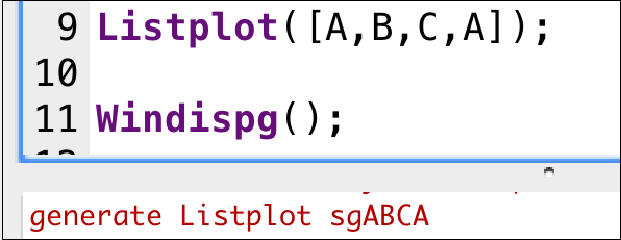
\includegraphics[bb=0.00 0.00 298.02 115.01,width=6cm]{Fig/pdtoconsole.pdf} \end{center}

プロットデータの内容は,Cindyscriptの println() 関数を用いてコンソールに表示することができる。たとえば上記の場合,

\hspace{10mm}  \verb|println(sgABCA)|
        
とすると,

\hspace{10mm}  \verb| [[1,3],[-1,0],[3,0],[1,3]] |

と表示される。A,B,C,A のそれぞれの座標からなるリストである。

プロットデータは,Cindyscriptによるプログラムで作成してそれを\ketcindy で利用することもできる。( \hyperlink{listplot}{Listplot()の例}  を参照)ただし,要素の数が大きいとエラーとなるので,1つのプロットデータの要素は200程度とするのがよい。これより多い場合は分割する。

\newpage
%======= Cindyscript ===========

\section{Cindyscript}
\subsection{Cindyscriptエディタ}
CindyscriptはCinderellaのプログラミング言語で,Cinderella上のスクリプトエディタで記述する。スクリプトエディタは,「スクリプト」メニューの「Cindyscript」を選択するか,Ctrl+9 (Windows) / ⌘+9 (Mac) で開く。\\
\vspace{110mm}
\begin{layer}{150}{0}
\putnotese{5.5}{15}{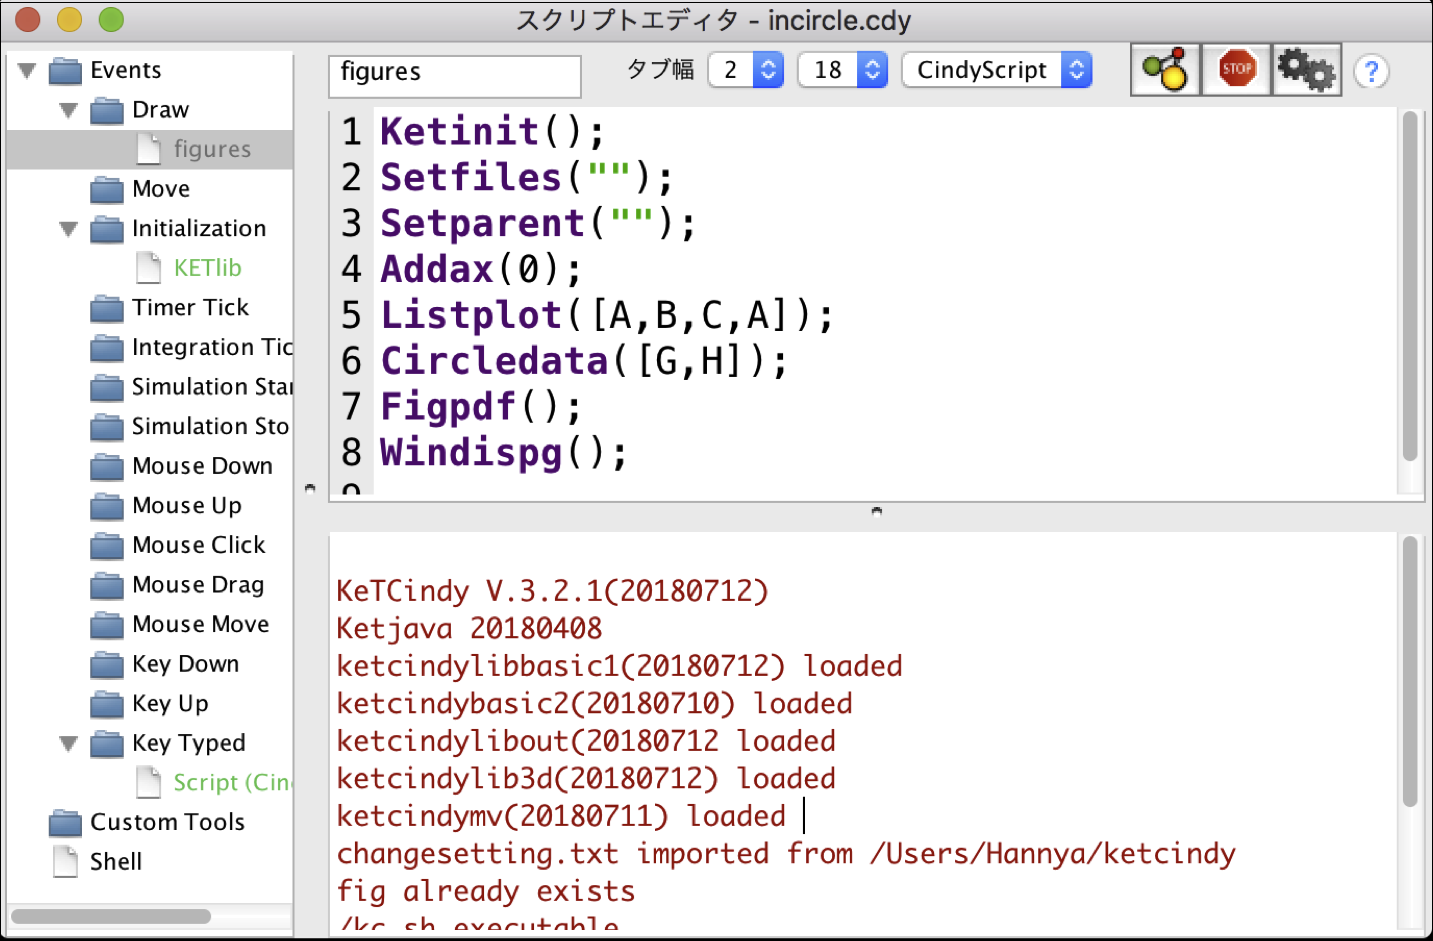
\includegraphics[bb=0.00 0.00 687.84 451.68,width=12.5cm]{Fig/slot.pdf}}
\arrowlineseg[16]{20}{20}{10}{90}
\putnotese{15}{5}{スロット}
\arrowlineseg[16]{40}{20}{10}{100}
\putnotese{32}{5}{ページ名}
\arrowlineseg[16]{80}{20}{15}{140}
\putnotese{50}{5}{フォントサイズ}
\arrowlineseg[16]{107}{20}{15}{140}
\putnotese{80}{5}{描画面を前面に}
\arrowlineseg[16]{120}{20}{10}{110}
\putnotese{110}{5}{実行}
\arrowlineseg[16]{125}{20}{10}{90}
\putnotese{120}{5}{ヘルプ}
\putnotese{90}{35}{メインウィンドウ}
\putnotese{90}{65}{コンソール}
\end{layer}

スロットはそれぞれの実行タイミングでスクリプトを実行するものであり,他のプログラミング言語にはない特徴である。(スロットが隠れているときは境界線をドラッグする)

よく使うスロットは次の通り。

\begin{tabbing}
123456789012345678\=\kill
Draw \>描画面になにか変化が起きる(点を動かすなど)と実行される。\\
 \>通常はここにスクリプトを書く。ひな形の templatebasic1.cdy では,\\
 \>Ketinit() などが記述された figures ページが用意されている。\\
Initialization \>スクリプトを実行すると、始めに1度 だけ実行される。\\
 \>したがって,関数定義や変数の初期設定などを書く。\\
 \>ひな形の templatebasic1.cdy ではここに KETlib というページがあり,\\
 \>\ketcindy の初期設定に関する記述がある。\\
Key Typed   \>キーボードが押されたとき実行される。\\
   \> KeTCindyでは,ボタンによらずキーボードで出力を行うための\\
   \>スクリプトが書かれている。
\end{tabbing}

1つのスロットに複数のページを作ることができる。たとえば,KETlib以外に初期設定のスクリプトを書く場合は,Initialzation スロットのフォルダアイコンをクリックすることで新しいページができる。

KeTCindyの描画コマンドは Draw スロットに書く。

\vspace{\baselineskip}
{\bf  ページ名}

各スロットでは,ページを分けて記述することができる。各ページの名前はスクリプトエディタの上の欄に書くことができる。

\vspace{\baselineskip}
{\bf  フォントサイズ}

編集エリアのフォントサイズを変更する。

\vspace{\baselineskip}
{\bf  実行ボタン}

プログラムを実行する。プログラムの実行は Shift+Enter でもできる。

\vspace{\baselineskip}
{\bf  ヘルプボタン}

ブラウザを開いてマニュアルを表示する。

\vspace{\baselineskip}
{\bf  コンソール}

print() 関数の結果やエラーメッセージが表示する。エラーメッセージは,「WARNING:」または「syntax error」に続いてその内容と該当する行番号が示される。これを読んでスクリプトの書き間違いをチェックする。

\subsection{スクリプトの記述}
編集エリアにプログラムを書くと,文字が色分けされて表示される。組み込み関数は青,ユーザー定義関数は紫,定義されていない関数は赤,文字列は緑で表示される。KeTCindyの関数はユーザー定義関数なので紫色で表示される。

編集エリアでは,Ctrl+C と Ctrl+V によるコピーアンドペースト,Ctrl+X と Ctrl+V によるカットアンドぺーストができる。他のテキストエディタなどとの間でのコピーも同様にできる。

文字列の選択はマウスドラッグまたは Shift+カーソルキーでおこなえる。

Ctrl+F による検索はできない。

スクリプトを記述するときの基本的なルールは次の通り。

\vspace{\baselineskip}
・基本的に小文字で書く。大文字と小文字は区別される。

\hspace{5mm}\ketcindy では,Cindyscriptに組み込みの変数名・関数名と区別しやすいように,

\hspace{5mm}次の規則により名前を付けている。

\hspace{5mm}・グローバルな変数はすべて大文字か,大文字で始まるものとする。

\hspace{5mm}・局所変数は小文字で,関数定義の冒頭で regional() により局所変数として宣言する。

\hspace{5mm}・関数名は大文字で始まる。

・複数の半角スペースは無視され,一つの半角スペースと見なされる。

・行末にはセミコロンを書く。改行だけでは命令文の終わりにならない。

\subsection{変数と定数}
\vspace{\baselineskip}
{\bf  変数}

Cindyscriptでは,変数の型の宣言は不要。使用されたときに何が代入されたかで自動的に型が決まり,さらに,宣言し直さなくても異なる型の値を代入することができる。

\vspace{\baselineskip}

【例】
\begin{verbatim}
    a=10;
    b=2;
    c=a+sqrt(b);
    a="の平方根";
    println("10に "+b+a+" を加えると"+c);
\end{verbatim}

この例では,始めにaは整数型であるが,4行目で文字列に変わる。

文字列はダブルクウォートでくくる。異なる型の演算には注意を要するが,例外的に,5行目のように,文字列と数を+演算子で結ぶと,数は文字列化されて結合される。

\vspace{\baselineskip}
{\bf  予約定数}

Cindyscriptでは,円周率 (pi) と虚数単位(i) が定数として予約されている。i は,変数として使用することもでき,そのような場合,虚数単位に戻すには  \verb|i=complex(0,1)| を実行する。

\vspace{\baselineskip}
{\bf KeTCindyの予約変数}

 \ketcindy  が内部的に使用する予約変数がある。そのうち次のものはユーザーが値を変更または設定することができる。
\begin{tabbing}
1234\=567890123\=45678989012345678901234567890123\=\kill
  \>Fhead  \>書き出されるファイル名の頭部。Setfiles() によって設定できる。\\
  \>Texparent  \>親プロセスのファイル名。Setparent()によって設定できる。\\
  \>Dirhead  \>パスの頭部\\
  \>Dirlib  \>ライブラリ ketlib のパス\\
  \>Dirbin  \>ketbin のパス\\
  \>Dirwork  \>作業ディレクトリのパス。Changework()によって設定できる。\\
  \>Shellfile  \>シェルファイル名
\end{tabbing}

以下の予約変数は,ライブラリが使用するグローバル変数であるので,ユーザーはこれらの変数に値を代入してはいけない。なお,変数は大文字小文字を区別するので,すべて小文字で書く分には支障はない。ユーザーが作るプログラムでは,すべて小文字か,先頭だけが大文字の変数を使うことを勧める。

\vspace{\baselineskip}
ADDAXES, ArrowlineNumber, ArrowheadNumber, BezierNumber, COM0thlist, COM1stlist, COM2ndlist, Dq, FUNLIST, Fnamesc ,Fnamescibody,Fnameout,Fnametex, GDATALIST, GLIST, GCLIST, GOUTLIST, KCOLOR, KETPICCOUNT,KETPICLAYER, LETTERlist, LFmark, MilliIn, PenThick,PenThickInit,  POUTLIST, SCALEX, SCALEY, SCIRELIST, SCIWRLIST, TenSize, TenSizeInit, ULEN, XMAX, XMIN, YaSize, YaThick,   YMAX, YMIN, VLIST


\vspace{\baselineskip}
{\bf  リスト}

リストとは,数や文字などを集めたもので,それぞれのものを「要素」といい,\verb|[ ]|の中にコンマで区切って記述する。要素は型を問わない。\ketcindy\ では,曲線を描くプロットデータが座標のリストであり,リスト処理をうまく使えば \ketcindy\ で効率的に作図ができる。

リストのn番目の要素にアクセスするのに,アンダーバー\_ を使う。

\begin{verbatim}
  list=[1,2,3,4,5];
  println(list_2);
\end{verbatim}
とすると,list の中の2番目の要素 2 が表示される。
\begin{verbatim}
  list=[1,2,3,4,5];
  list_2="a";
\end{verbatim}
とすると,list の中の2番目の要素が文字 a に変わる。

たとえば,曲線の交点を求める \hyperlink{intersectcrvs}{Intersectcrvs()} の戻り値から交点の座標を求めるにはアンダーバーを使う。使用例は,Intersectcrvs() の例を参照されたい。

\subsection{よく使うCindyscriptのコマンド}
\vspace{\baselineskip}
{\bf 値の表示}

print(値)   :コンソールに値を表示する。改行しない。

println(値) :コンソールに値を表示する。改行する。

\vspace{\baselineskip}
【例】関数Intersectcrvs() の戻り値を表示する。
\begin{verbatim}
    tmp=intersectcrvs("sgAB","crCD");
    println(tmp);
\end{verbatim}

\vspace{\baselineskip}
{\bf 条件判断}

if(A,B,C)  : もしAが真なら(成り立てば)Bを,偽ならCを実行する。

Aの条件判断には次のものがよく使われる。
 \begin{tabbing}
1234\=56789012345678989012\=3456789012\=34567890123\=\kill
 \>  \verb|a|が\verb|b|より大きい \> \verb|if(a>b|,$\cdots$\\
 \>  \verb|a|が\verb|b|より小さい \> \verb|if(a<b|,$\cdots$\\
 \>  \verb|a|が\verb|b|以上  \> \verb|if(a>=b|,$\cdots$ (\verb|>|と=の順序に注意)\\
 \>  \verb|a|が\verb|b|以下  \> \verb|if(a<=b|,$\cdots$ (\verb|<|と=の順序に注意)\\
 \>  \verb|a|と\verb|b|が等しい \>  \verb|if(a==b|,$\cdots$ (等号を2つ)\\
 \>  \verb|a|と\verb|b|が異なる \> \verb|if(a!=b|,$\cdots$\\
\end{tabbing}

if 文はネストして使うことができる。

\vspace{\baselineskip}
  【例】n が正,負,ゼロのいずれかを判断して,コンソールに表示する。
\begin{verbatim}
    if(n>0,print("正"),if(n==0,print("0"),print("負")));
\end{verbatim}

\vspace{\baselineskip}
{\bf 繰り返し}

repeat(n,操作)    :操作をn回繰り返す。

repeat(n,s,操作)  :操作をn回繰り返す。カウンタとしてsを使う。(文字は他でも可)

\vspace{\baselineskip}
  【例】Aを4個並べて描画面に表示する。
\begin{verbatim}
    repeat(4,s,drawtext([s,0],4));
\end{verbatim}
  ここで,sの値は4回繰り返すうちに,1,2,3,4と変化する。

\vspace{\baselineskip}
{\bf リストによる繰り返し}

  forall(list,処理)  :リストの要素すべてに渡るように繰り返す。
  
\vspace{\baselineskip}
  【例】点のペアをリストとし,線分を描く。
\begin{verbatim}
    sglist=[[A,B],[C,D],[E,F]];
    forall(sglist,Listplot(#));
\end{verbatim}
  これは,
\begin{verbatim}
    Listplot([A,B]);
    Listplot([C,D]);
    Listplot([E,F]);
\end{verbatim}
とするのと同じ。ここで,\verb|#|は実行変数と呼ばれ,リストのそれぞれの要素を表す。

\vspace{\baselineskip}
{\bf ユーザー定義関数}

ユーザー定義関数は次の書式で定義する。

\hspace{10mm}関数名(引数):=(処理)

\vspace{\baselineskip}
【例】  引数の値の正負を表示する関数 sign(n) を定義する。
\begin{verbatim}
  sign(n):=(
    if(n>0,print("正"),print("0または負"));
   );
\end{verbatim}
定義した関数は
\begin{verbatim}
  n=3;
  println(sign(n));
\end{verbatim}
のようにして使う。

KeTCindyでは,アニメーションPDFを作成するときに,フレームを定義するのに使う。

\vspace{\baselineskip}
{\bf 幾何要素へのアクセス}

Cinderellaでは,点の座標は同次座標で表されており,点の名称でそのまま座標を取得できることが多い。そのため,たとえば Listplot() 関数では,点を指定するのに,座標 \verb|[a,b]| の代わりに点名を使うことができる。

\vspace{\baselineskip}
Listplot() の書式1  \verb|Listplot("1",[[1,1],[4,5]])|

Listplot() の書式2  \verb|Listplot("1",[A,B])|

\vspace{\baselineskip}

しかし,明確に直交座標で取得したい場合は  \verb|A.xy|(x,y 座標)  \verb|A.x|(x 座標 )   \verb|A.y|(y 座標)  として取得する。

\vspace{\baselineskip}
{\bf リスト処理}

Cindyscriptのリスト処理のうち,よく使うものを挙げる。

aからbまでの整数のリストは \verb|a..b| (ドット2つ)で生成できる。このリストの各要素を番号代わりに使って,\verb|apply(list,expr)| を用いると座標のリストを作ることができる。\verb|apply(list,expr)| は,\verb|list| の各要素に,処理 \verb|expr| を施したリストを作る関数である。

\vspace{\baselineskip}
【例】星形五角形を描く
\begin{verbatim}
    r=2;
    pt=apply(0..5,r*[cos(pi/2+#*4*pi/5),sin(pi/2+#*4*pi/5)]);
    repeat(5,s,Listplot(text(s),[pt_s,pt_(s+1)]));
\end{verbatim}

ここで,\verb|text(s)| は,数を文字列に変換するCindyscriptの組み込み関数。

\vspace{\baselineskip}
{\bf よくあるエラーメッセージ}
\begin{tabbing}
1234\=5678901234567890123456789\=\kill
 \>Index out of range \>リストの要素の個数外の値を指定した。\\
 \>String Index out of range \>文字列のインデックスが範囲外。\\
 \>Potential type mismatch \>変数の型が合わない。文字と実数をかけ算したときなど。\\
 \>unexpected ) \>括弧の種類が前後で合っていない。\\
 \>close  without open \>閉じ括弧に対応する開き括弧がない。\\
 \>open  without close \>開き括弧に対応する閉じ括弧がない。\\
 \>Unknown function \>関数が定義されていない。
\end{tabbing}


\vspace{\baselineskip}
その他,Cindyscriptについては,スクリプトエディタからヘルプを参照されたい。

\end{document}